% Intended LaTeX compiler: pdflatex
\documentclass[11pt]{article}
\usepackage[utf8]{inputenc}
\usepackage[T1]{fontenc}
\usepackage{graphicx}
\usepackage{grffile}
\usepackage{longtable}
\usepackage{wrapfig}
\usepackage{rotating}
\usepackage[normalem]{ulem}
\usepackage{amsmath}
\usepackage{textcomp}
\usepackage{amssymb}
\usepackage{capt-of}
\usepackage{hyperref}
\author{Liam Hurwitz}
\date{\today}
\title{Test Protokol}
\hypersetup{
 pdfauthor={Liam Hurwitz},
 pdftitle={Test Protokol},
 pdfkeywords={},
 pdfsubject={},
 pdfcreator={Emacs 26.3 (Org mode 9.4)}, 
 pdflang={English}}
\begin{document}

\maketitle
\newpage
\tableofcontents

\newpage
\section{Anleitung}
Diese Test Protocoll basiert sich an der C4 test Abdekung, dann versuchen wir jedes Varientes an unsere Software zu testen.

\section{Login Screen}

\label{sec:orgc5dc561}
\subsection{Registrierung}
Auf diesem Bildschirm kann sich der Benutzer anmelden, dazu ist es notwendig, dass der User eine Passwort und Name gibt.\\
\begin{figure}[htp]
\centering
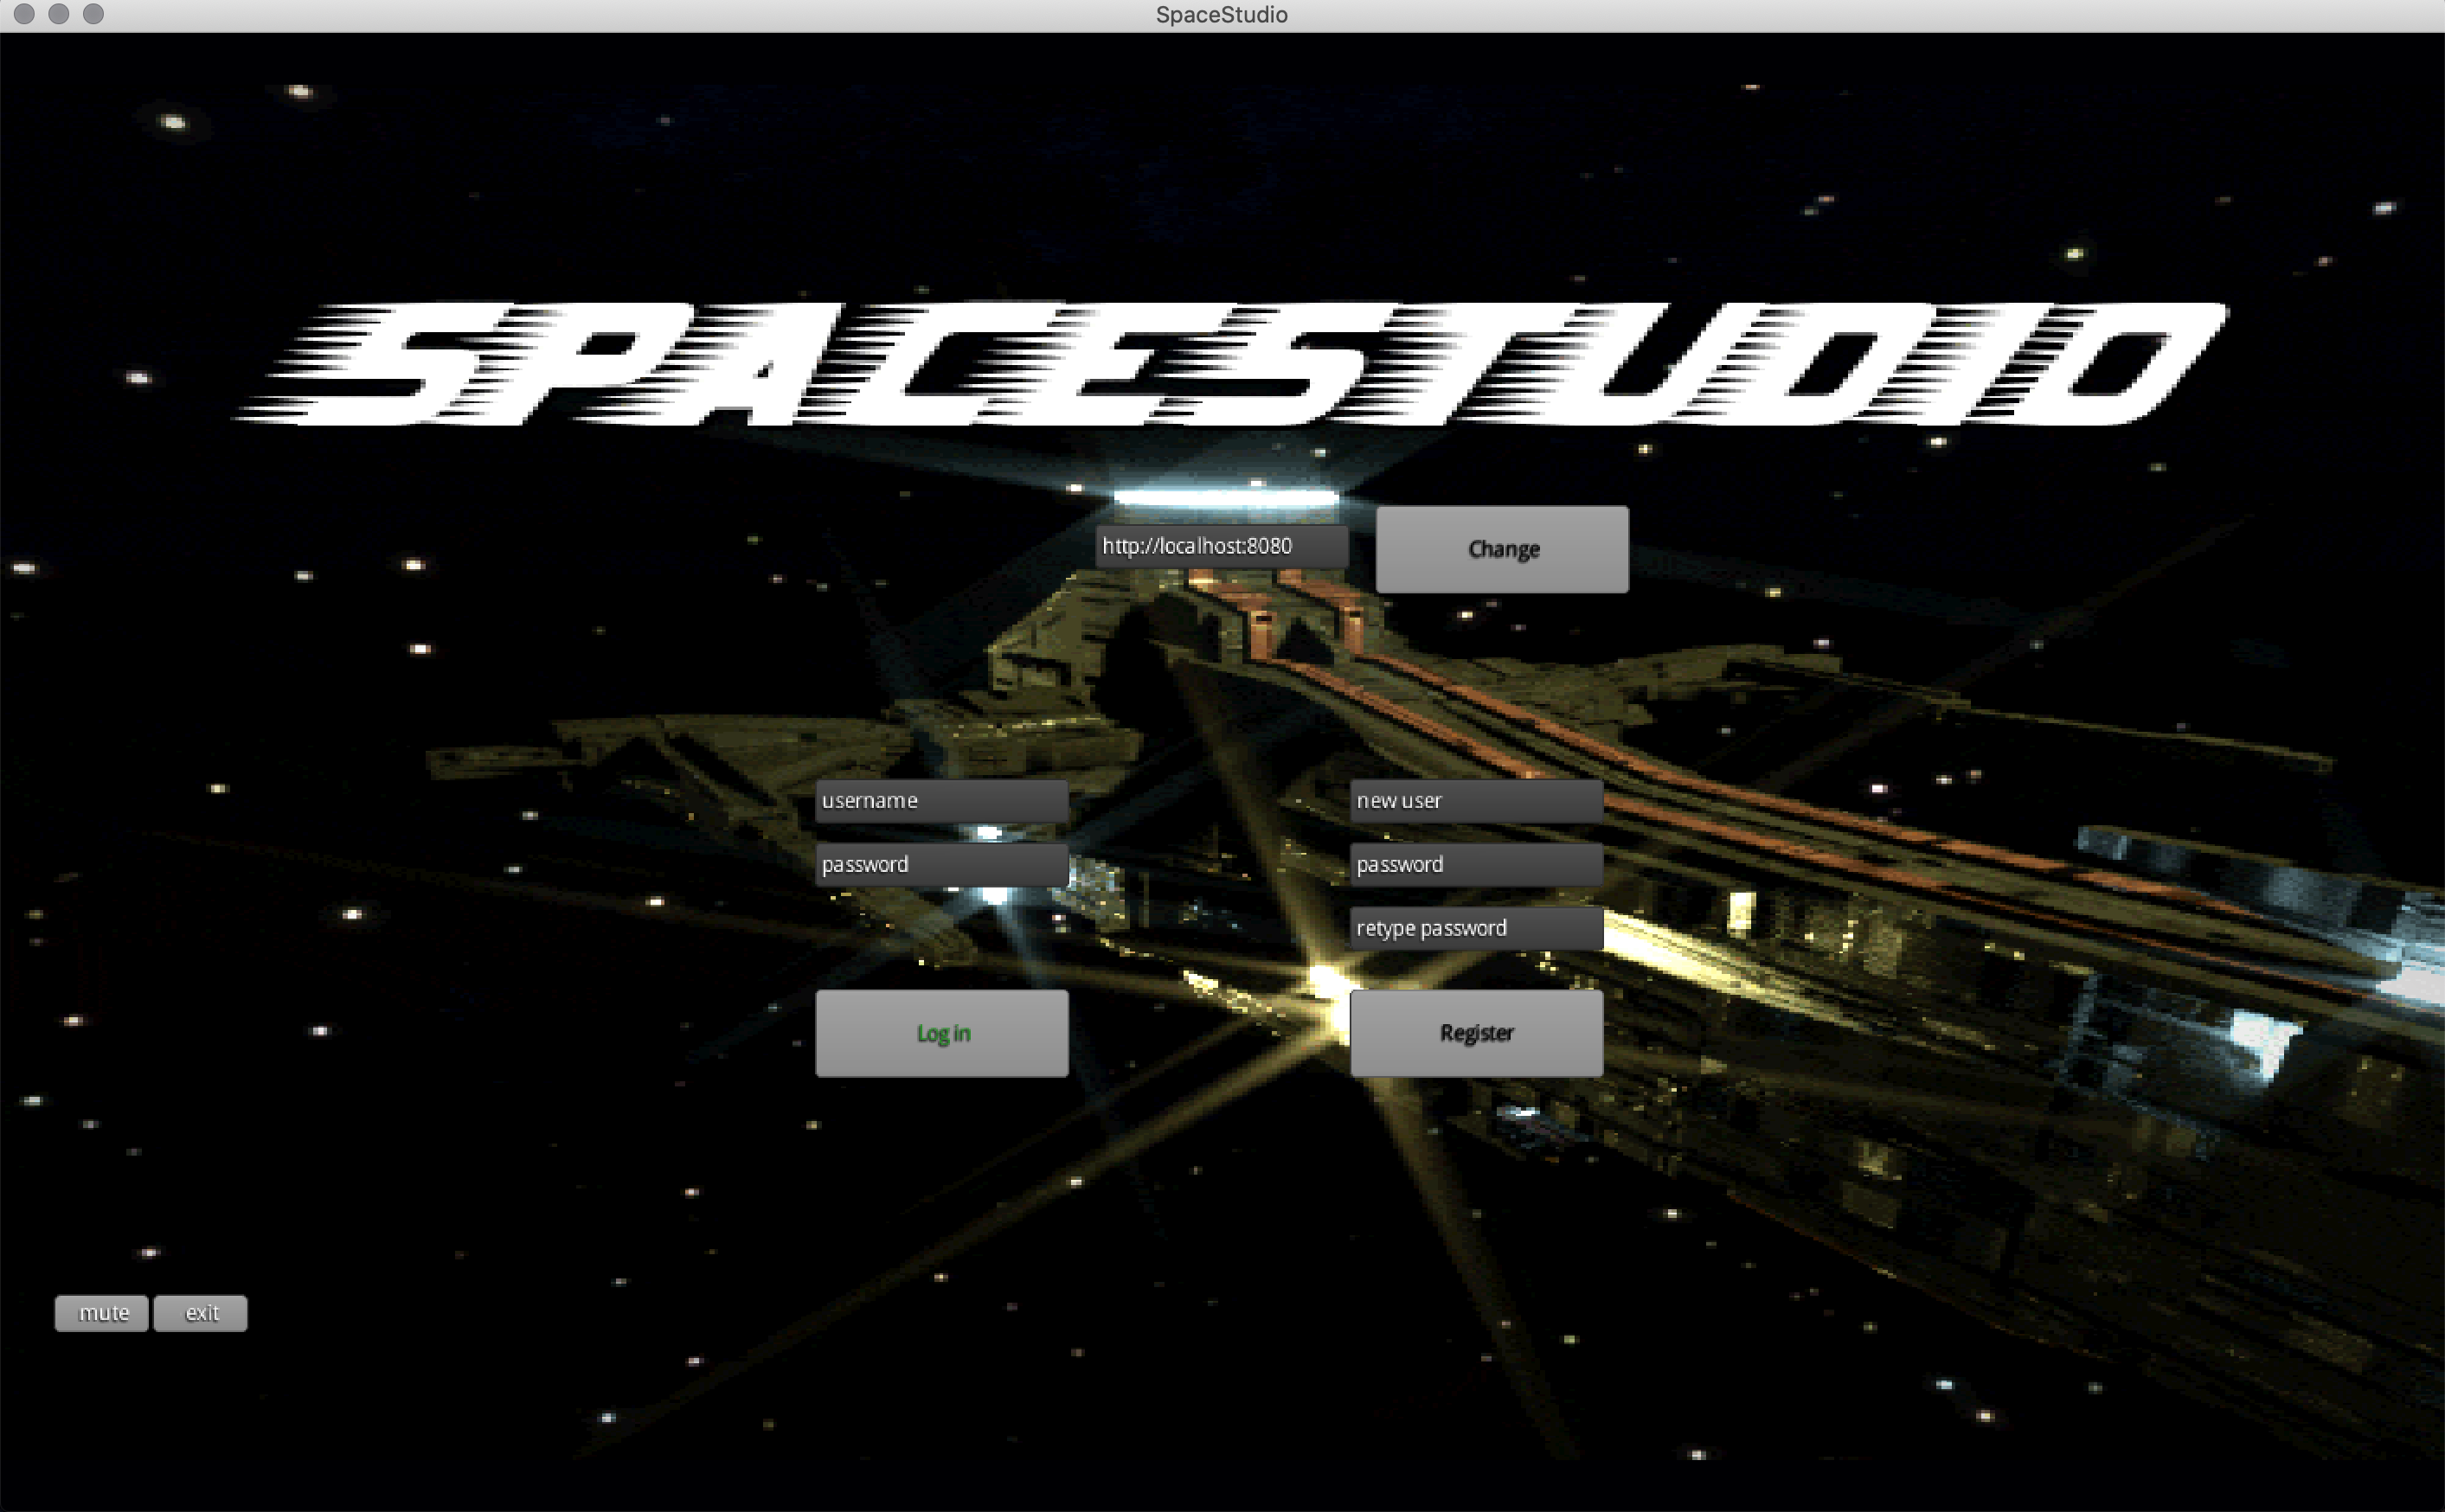
\includegraphics[scale=0.3]{TestProtocolBilder/startScreen.png}
\caption{Start Screen}
\end{figure}

\newpage
\subsubsection{falsche/erfolgreiche  Registrierung}
Wenn der Benutzer die Felder korrekt eingegeben hat, erhält er eine grüne Nachricht, in der sich die Bestätigungsnachricht des Servers für die Erstellung seiner Instanz befindet.\\
\begin{figure}[h]
\centering
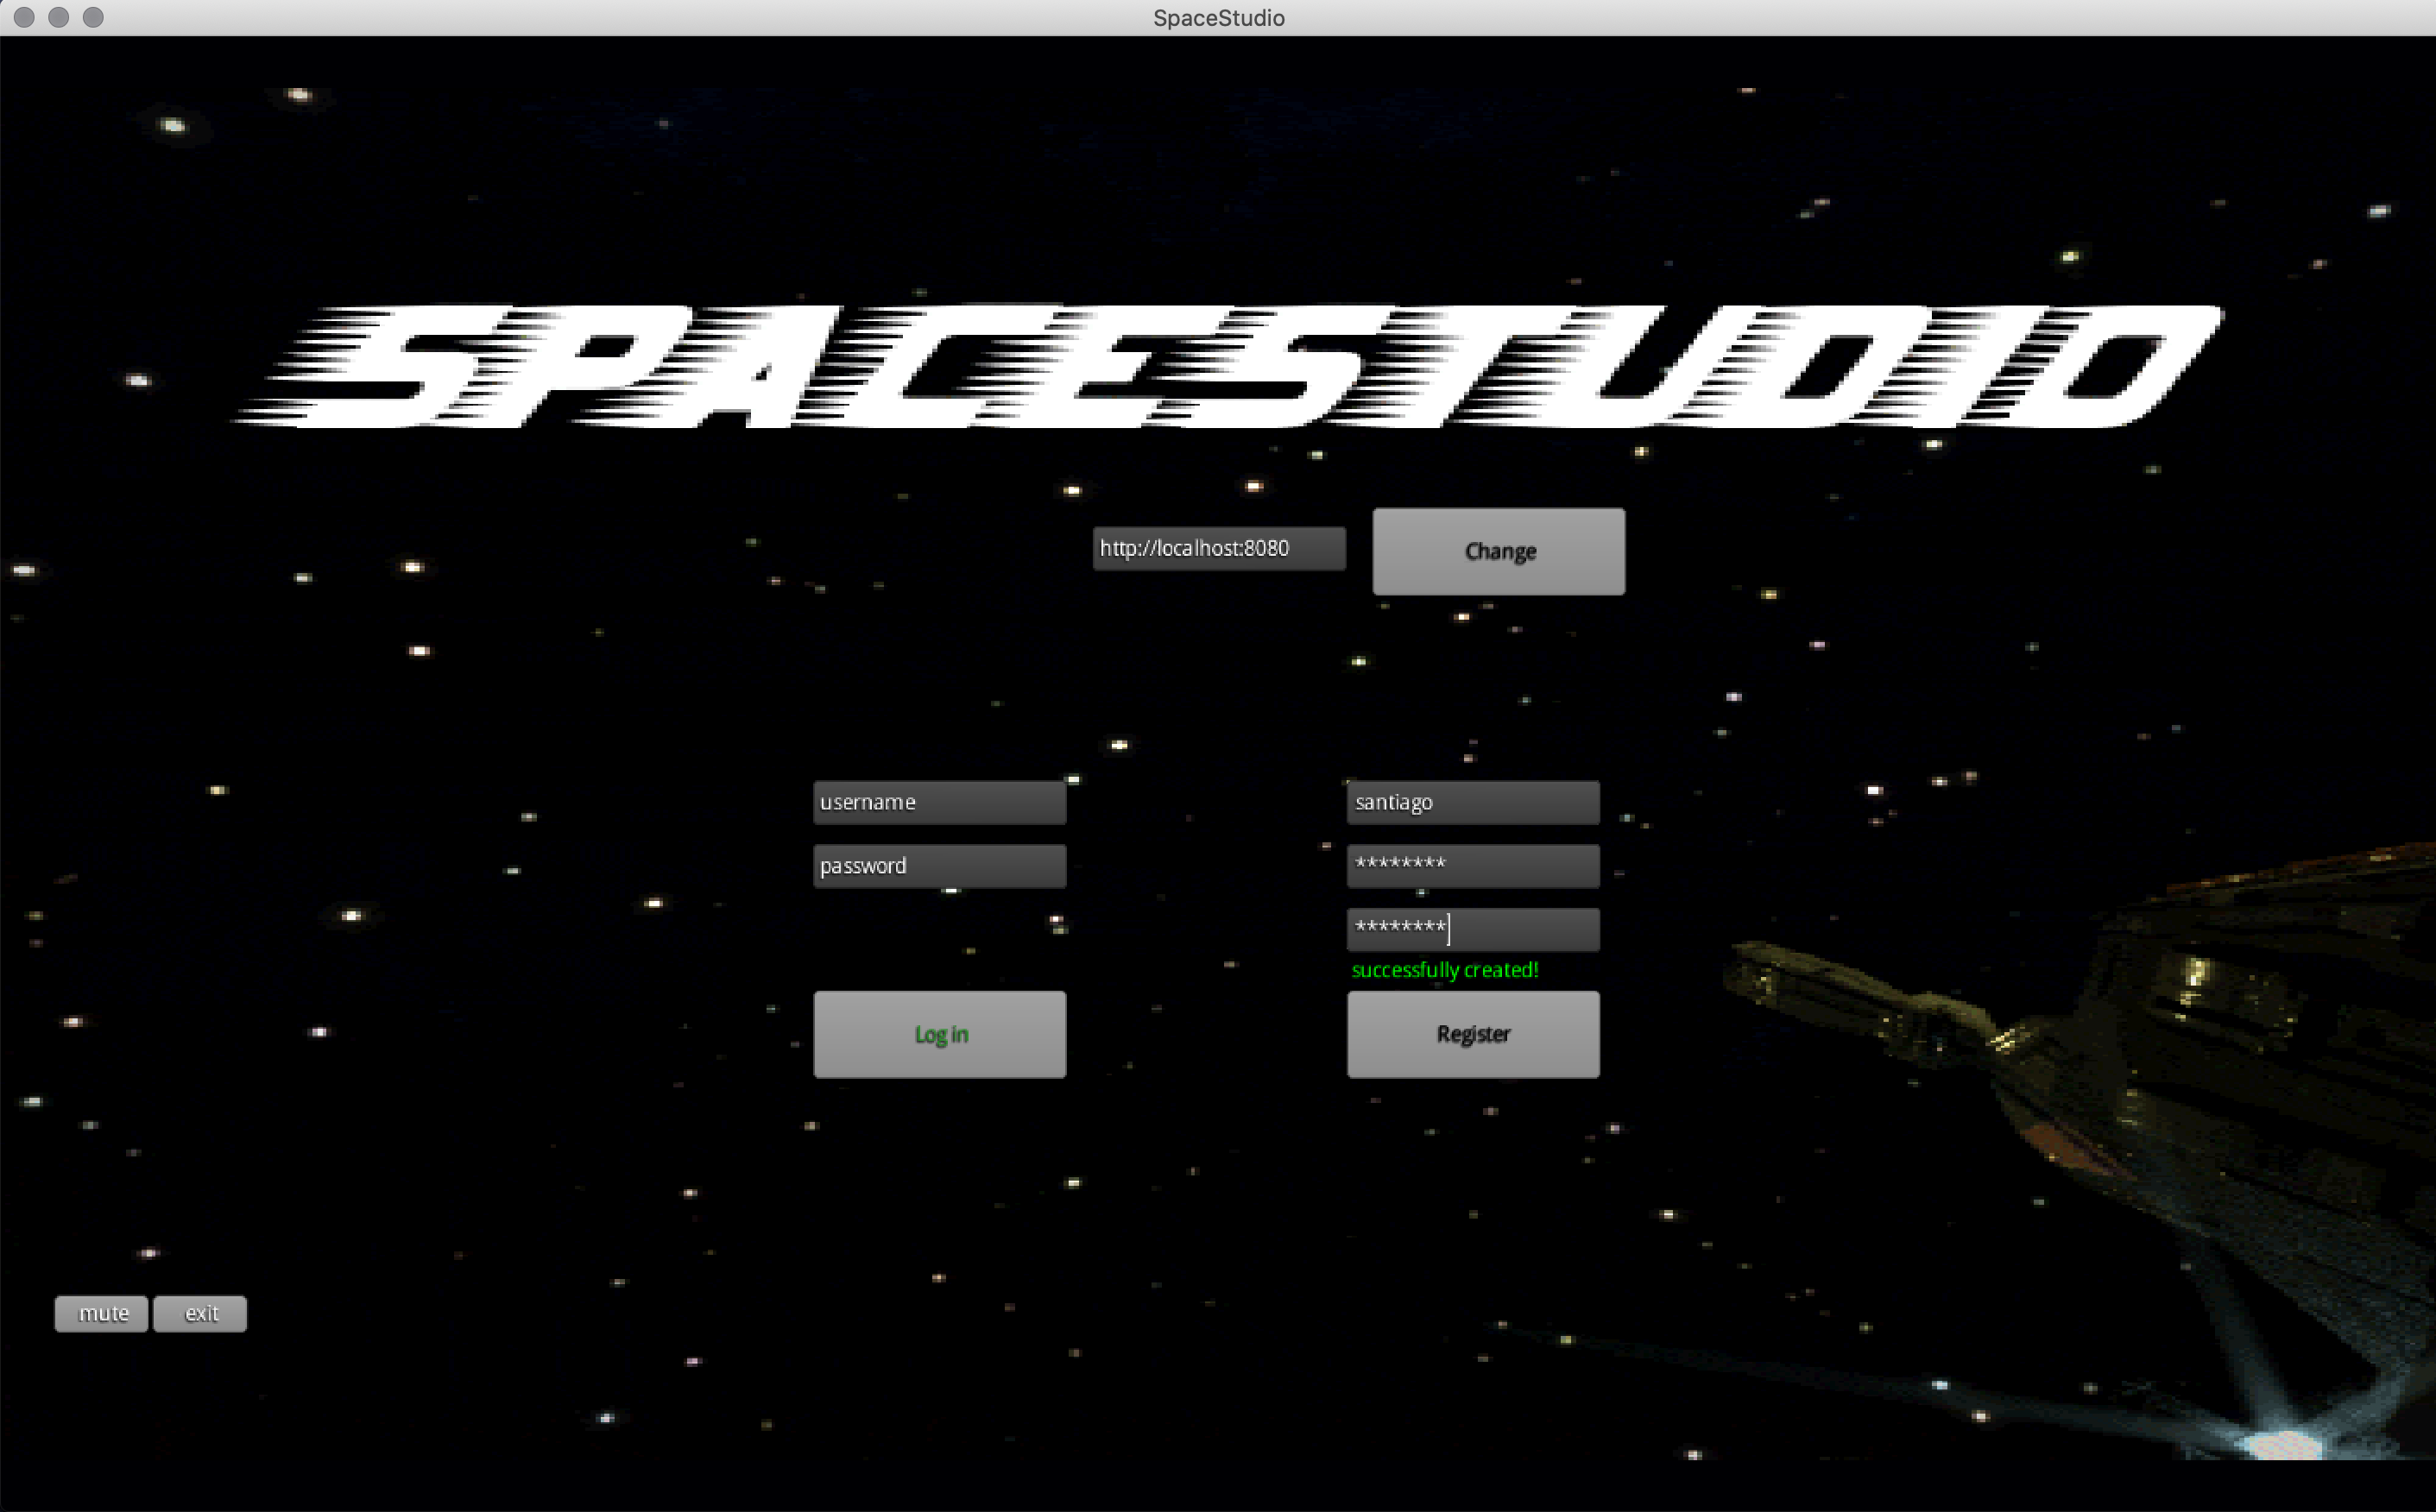
\includegraphics[scale=0.3]{TestProtocolBilder/erfolgAnmelden.png}
\caption{Erfolg Anmelden}
\end{figure}

Wenn der Benutzer fehlerhafte, wiederholte oder unvollständige Daten in den Registrierungsteil schreibt, erhält er eine negative Bestätigungsmeldung, in der das Problem erläutert wird, auf das der Server beim Speichern der Daten gestoßen ist.\\
\begin{figure}[h]
\centering
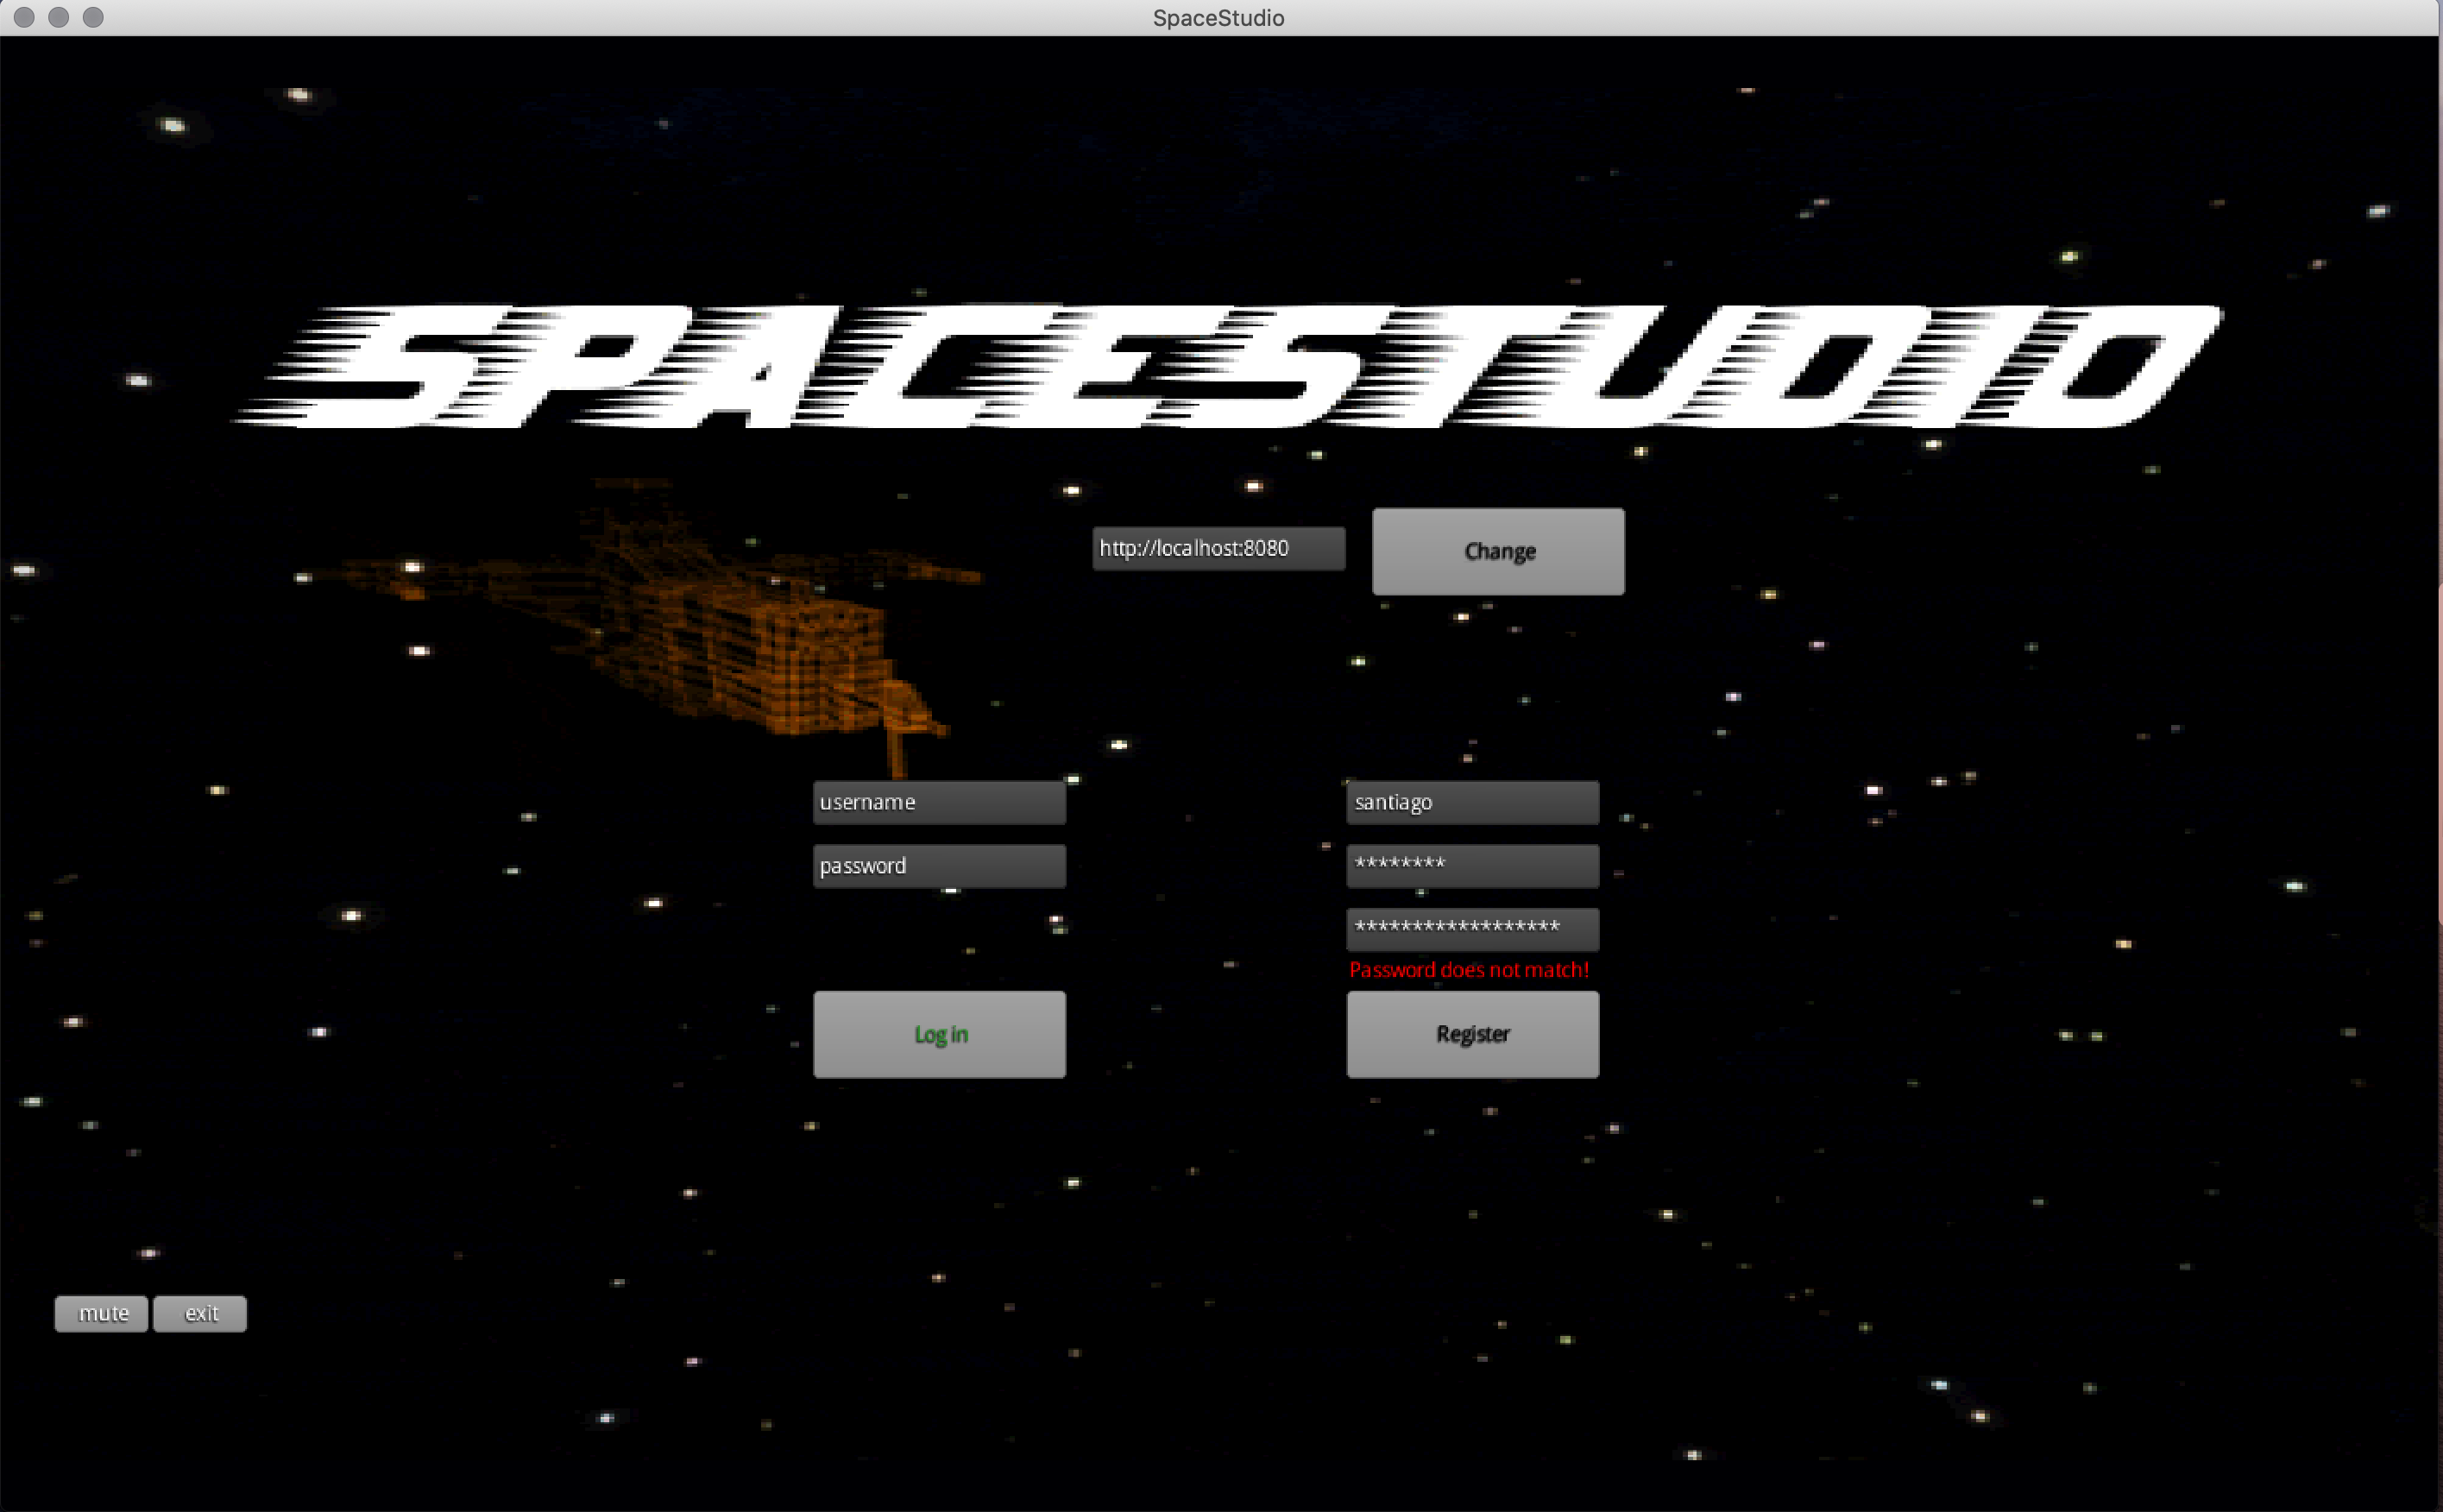
\includegraphics[scale=0.3]{TestProtocolBilder/doesnotMatchPassword.png}
\caption{ungultiges Password order Name}
\end{figure}
\newpage
\subsubsection{erfolgreiche  Registrierung}
Wenn sich der Benutzer mit dem richtigen Namen und Passwort registriert hat, überprüft der Server die Daten und der Benutzer wird zum Menübildschirm gesendet.\\

\begin{figure}[h]
\centering
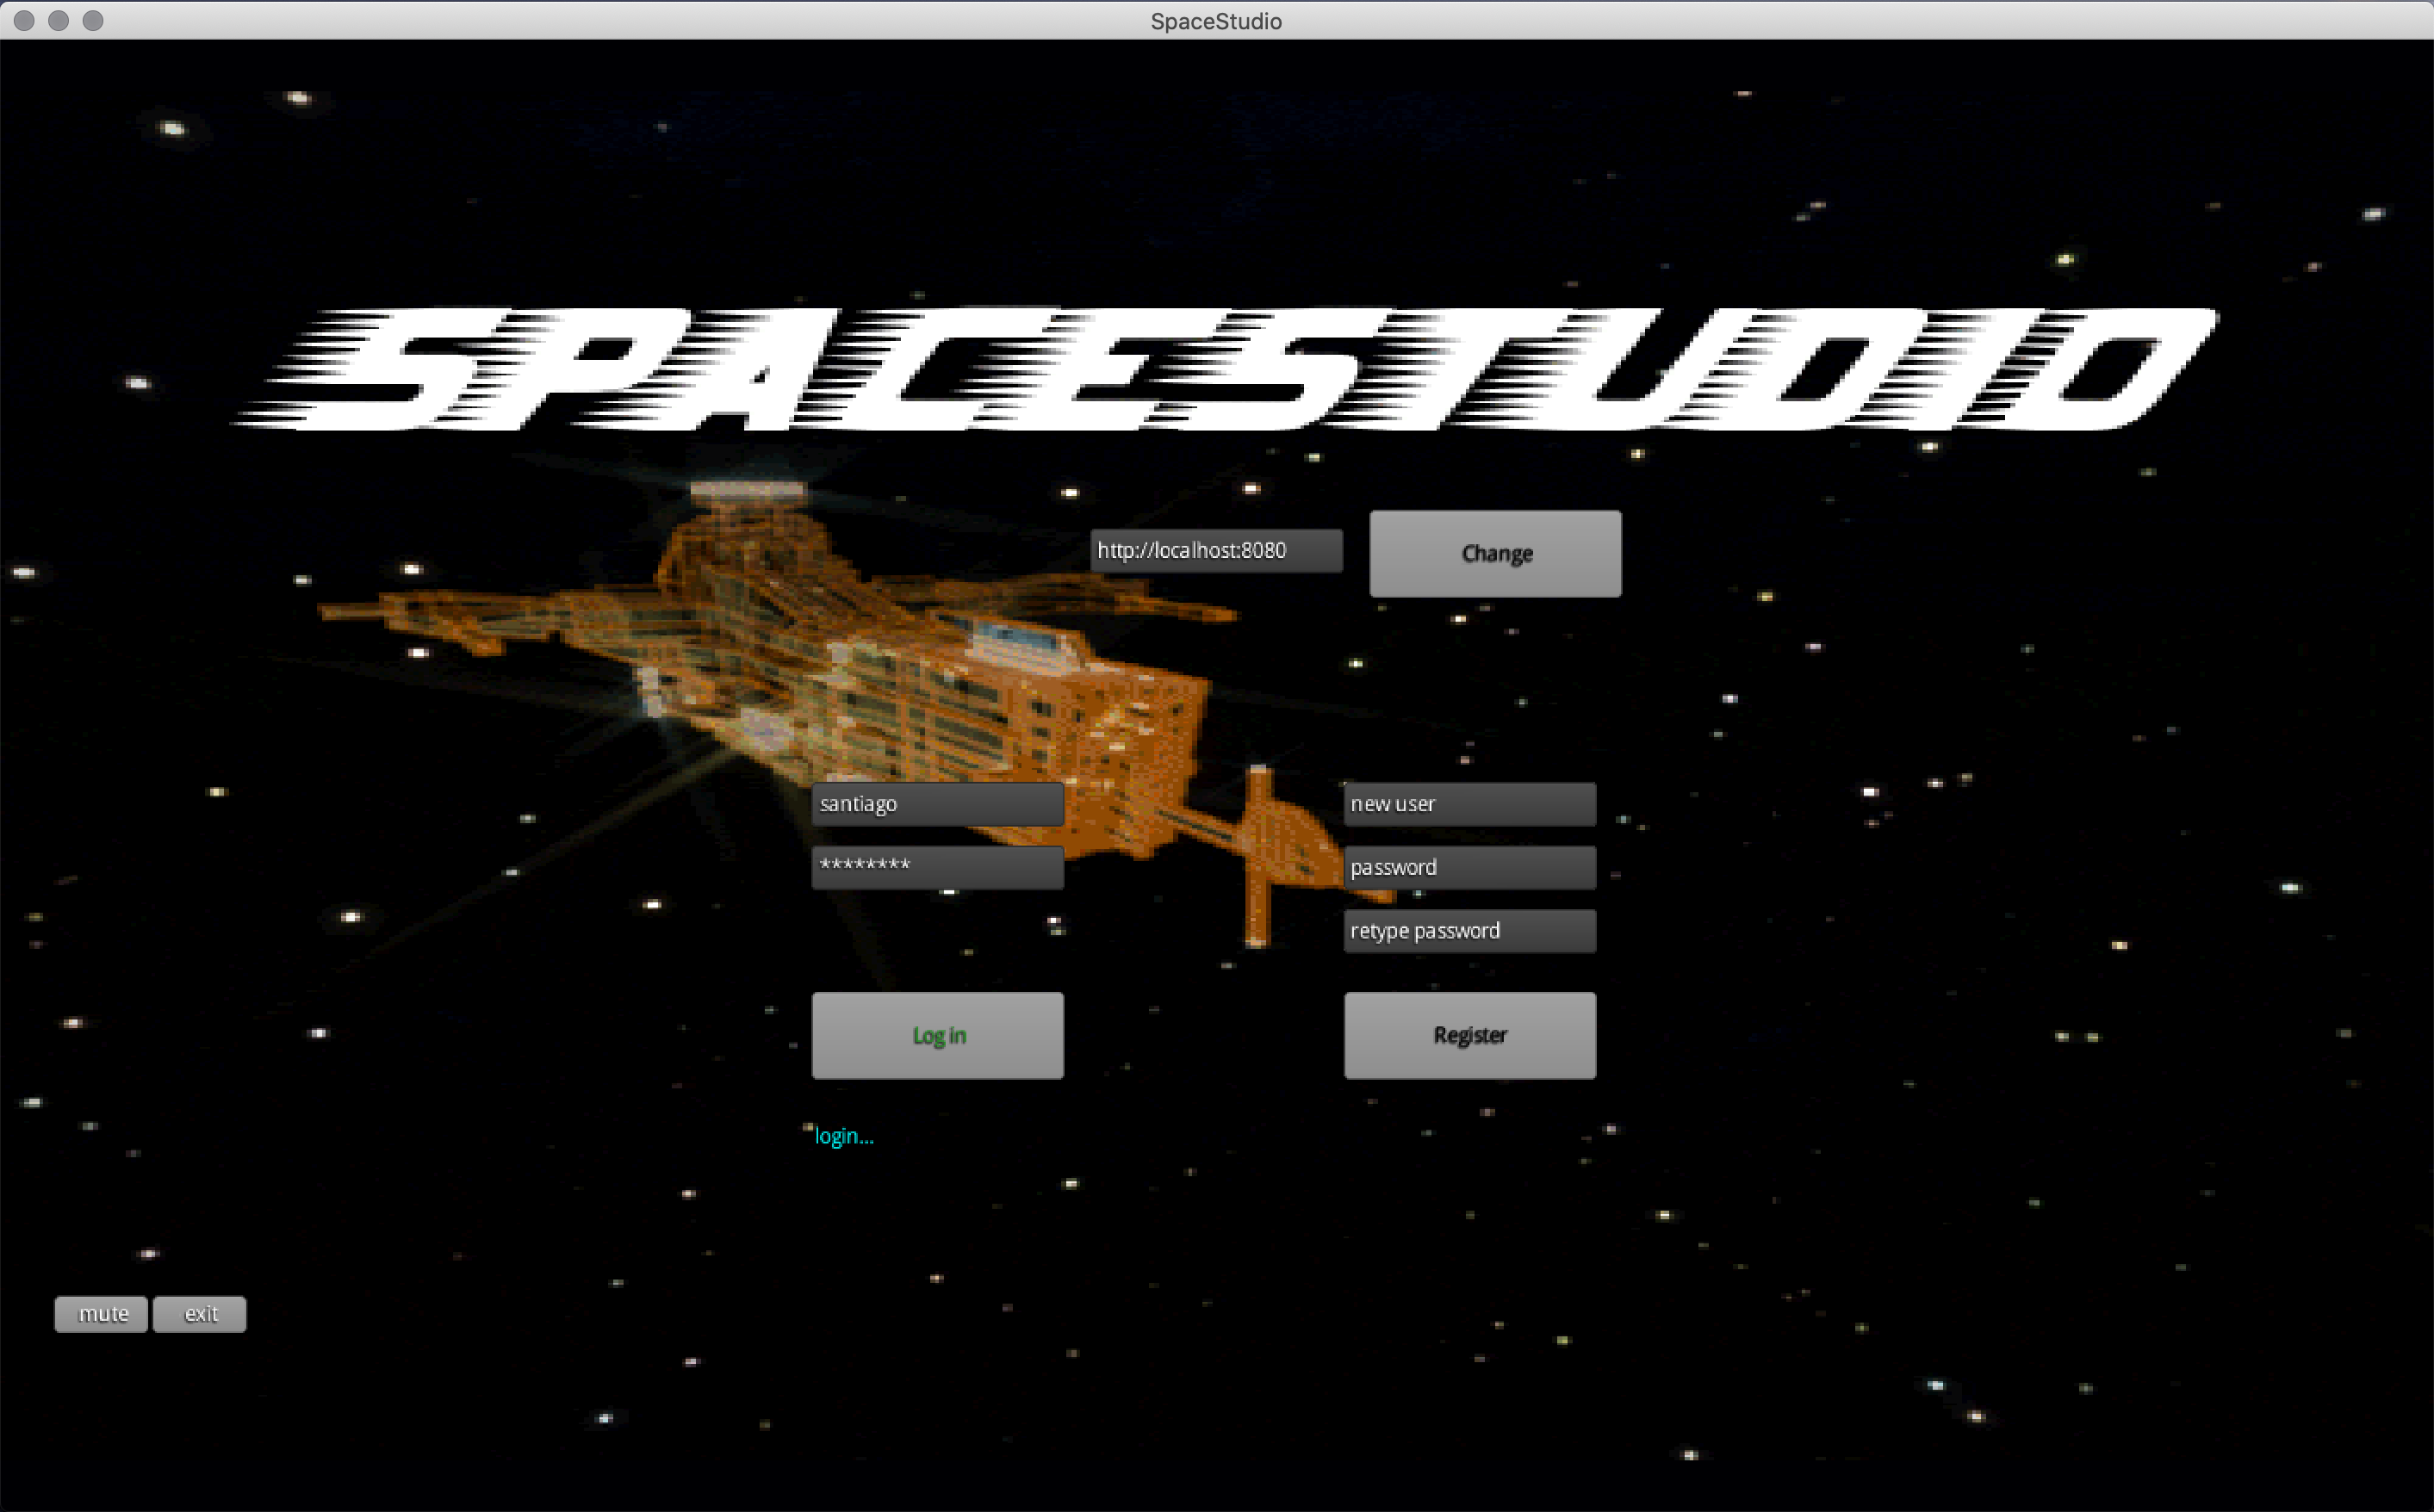
\includegraphics[scale=0.3]{TestProtocolBilder/erfolgLogin.png}
\caption{Login Erfolg}
\end{figure}
\newpage
\subsection{Anmeldung}
\subsubsection{ falsche Anmeldung}
Wenn sich der Benutzer mit falschen Daten angemeldet hat, kann der Server den Benutzer nicht validieren, sodass er nicht zum nächsten Bildschirm gesendet werden kann.
\begin{figure}[h]
\centering
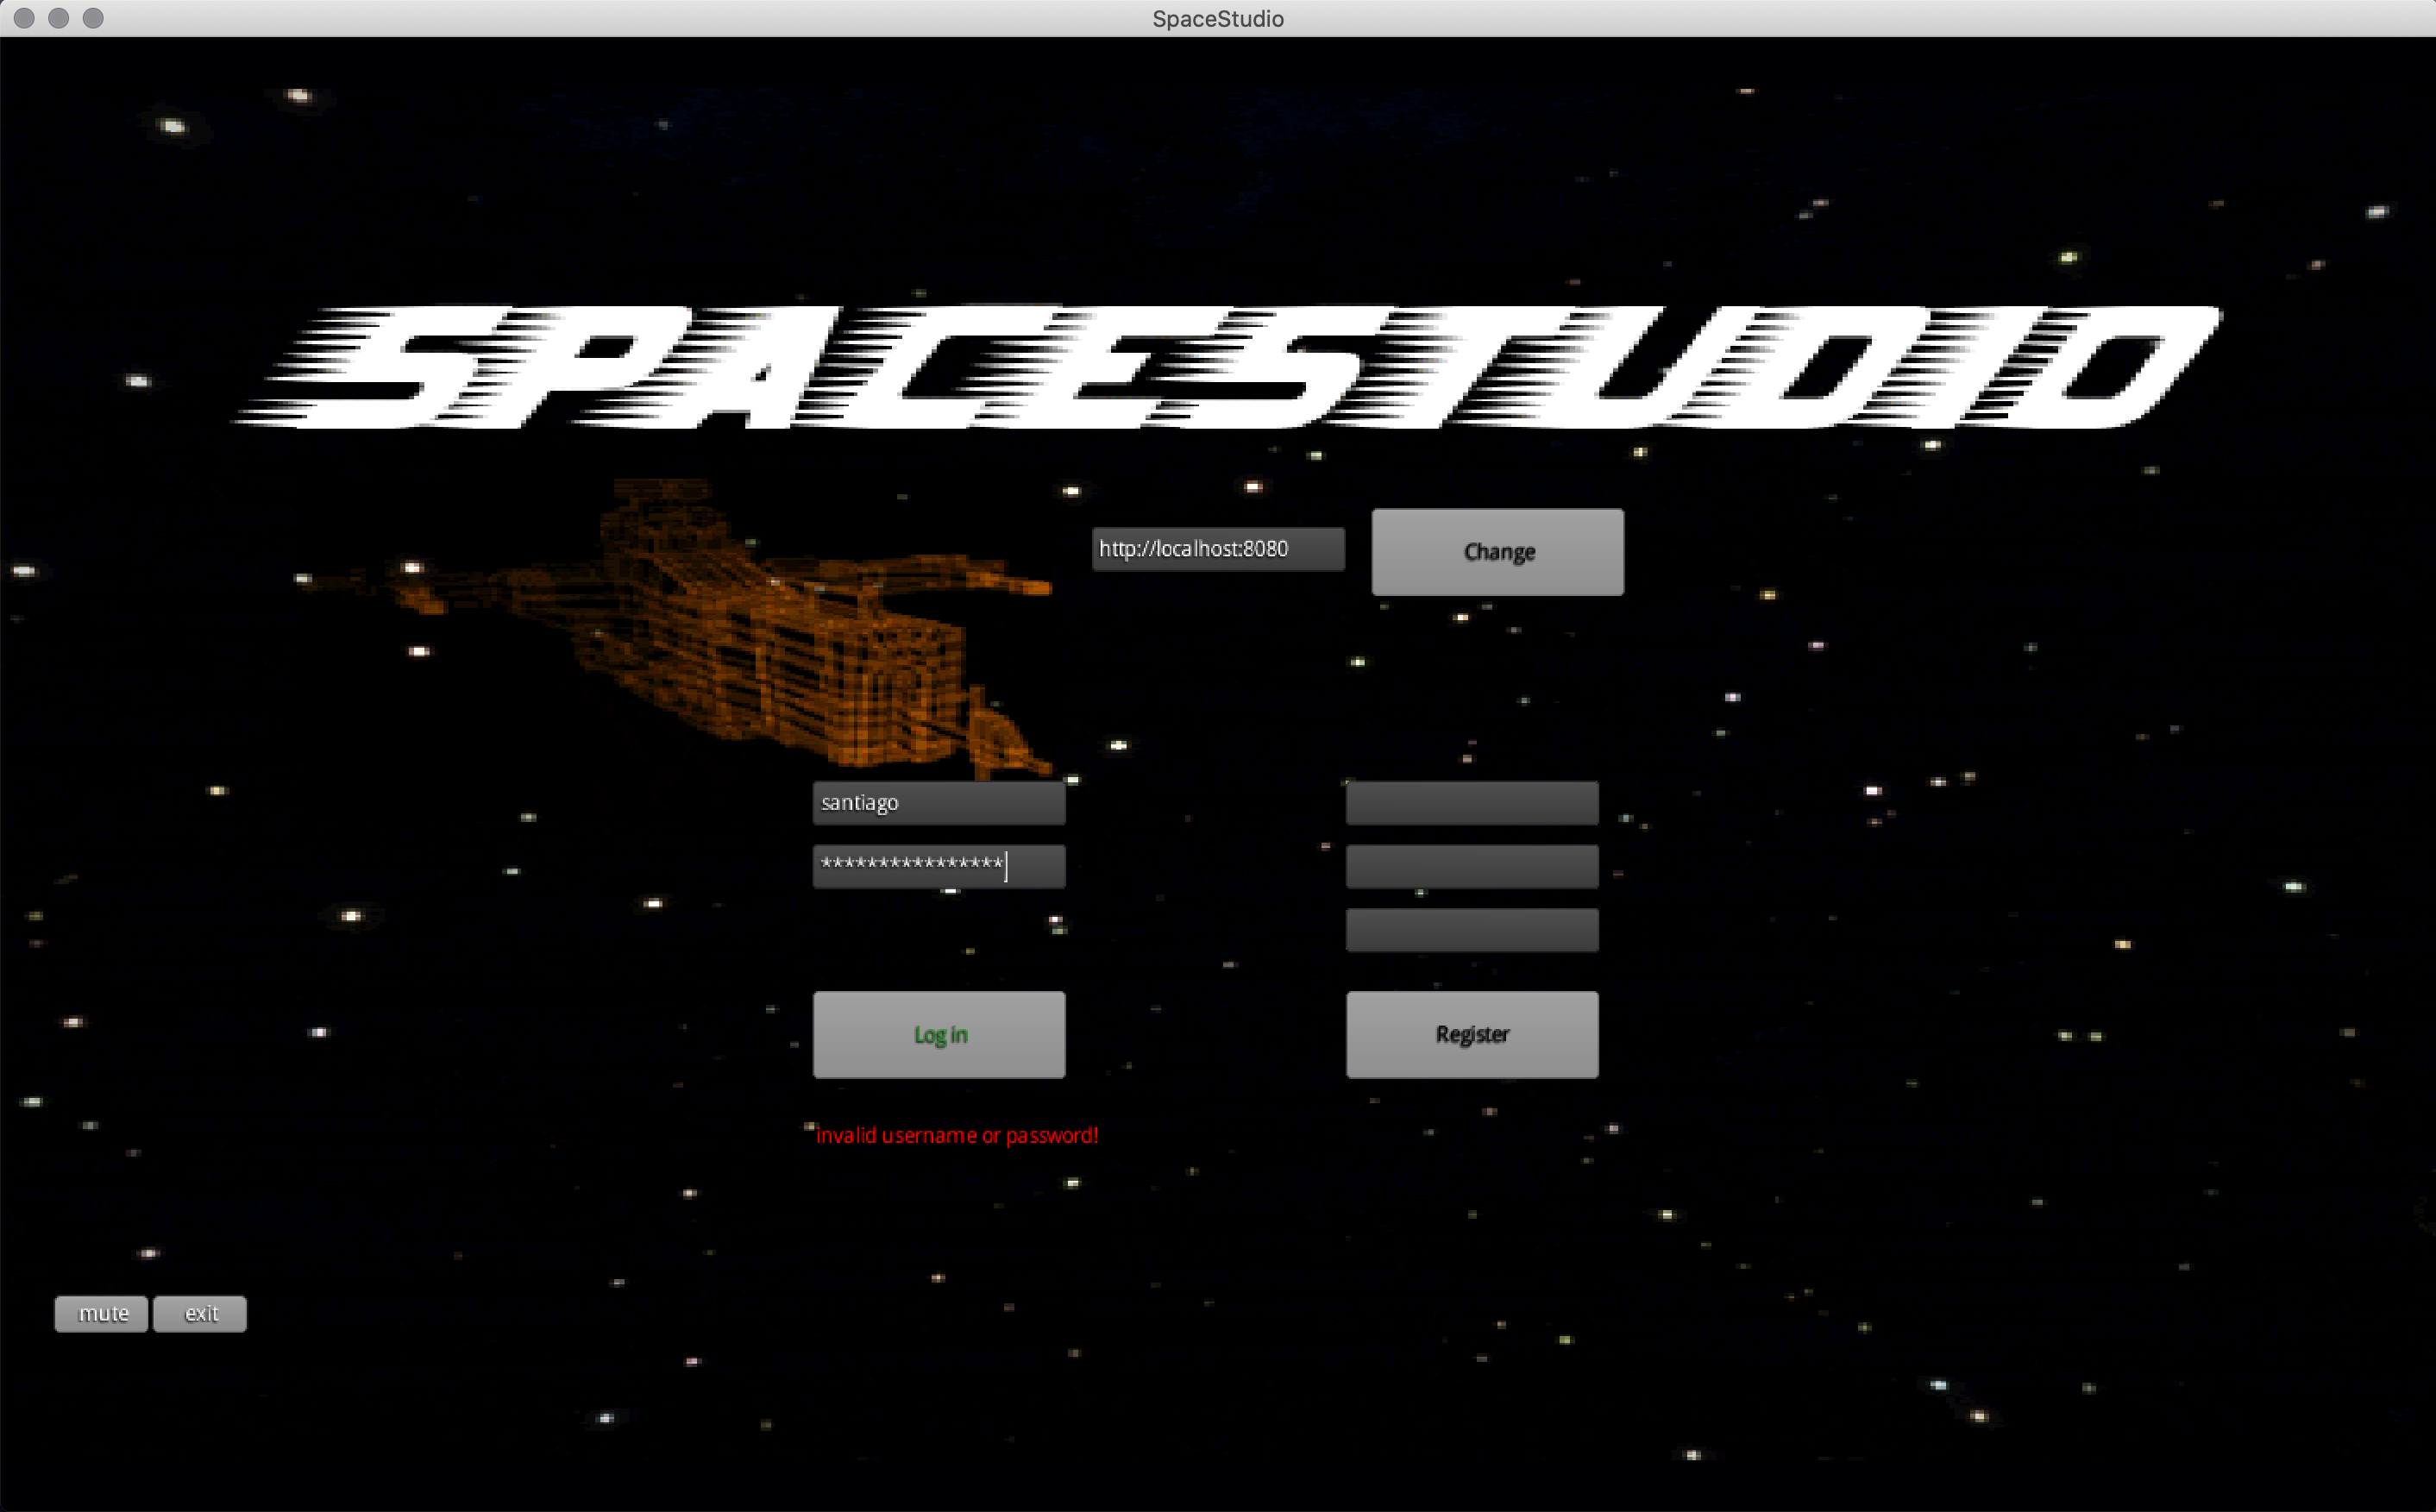
\includegraphics[scale=0.3]{TestProtocolBilder/invalidCredentials.png}
\caption{ungültiges Zugangsdaten}
\end{figure}
\newpage
Wenn sich der Benutzer mit den richtigen Anmeldeinformationen anmeldet, wird der Benutzer zum Menübildschirm weitergeleitet.\\

\section{Menu Screen}
Auf dem Menübildschirm sind die Optionen:
\begin{itemize}
\item New Game: Mit dieser Option kann der Benutzer ein neues Spiel starten
\item About: In dieser Option können Informationen zu den Entwicklern gefunden werden.
\item Exit: Mit dieser Option kann der Benutzer das Spiel beenden.
\end{itemize}
\begin{figure}[htp]
\centering
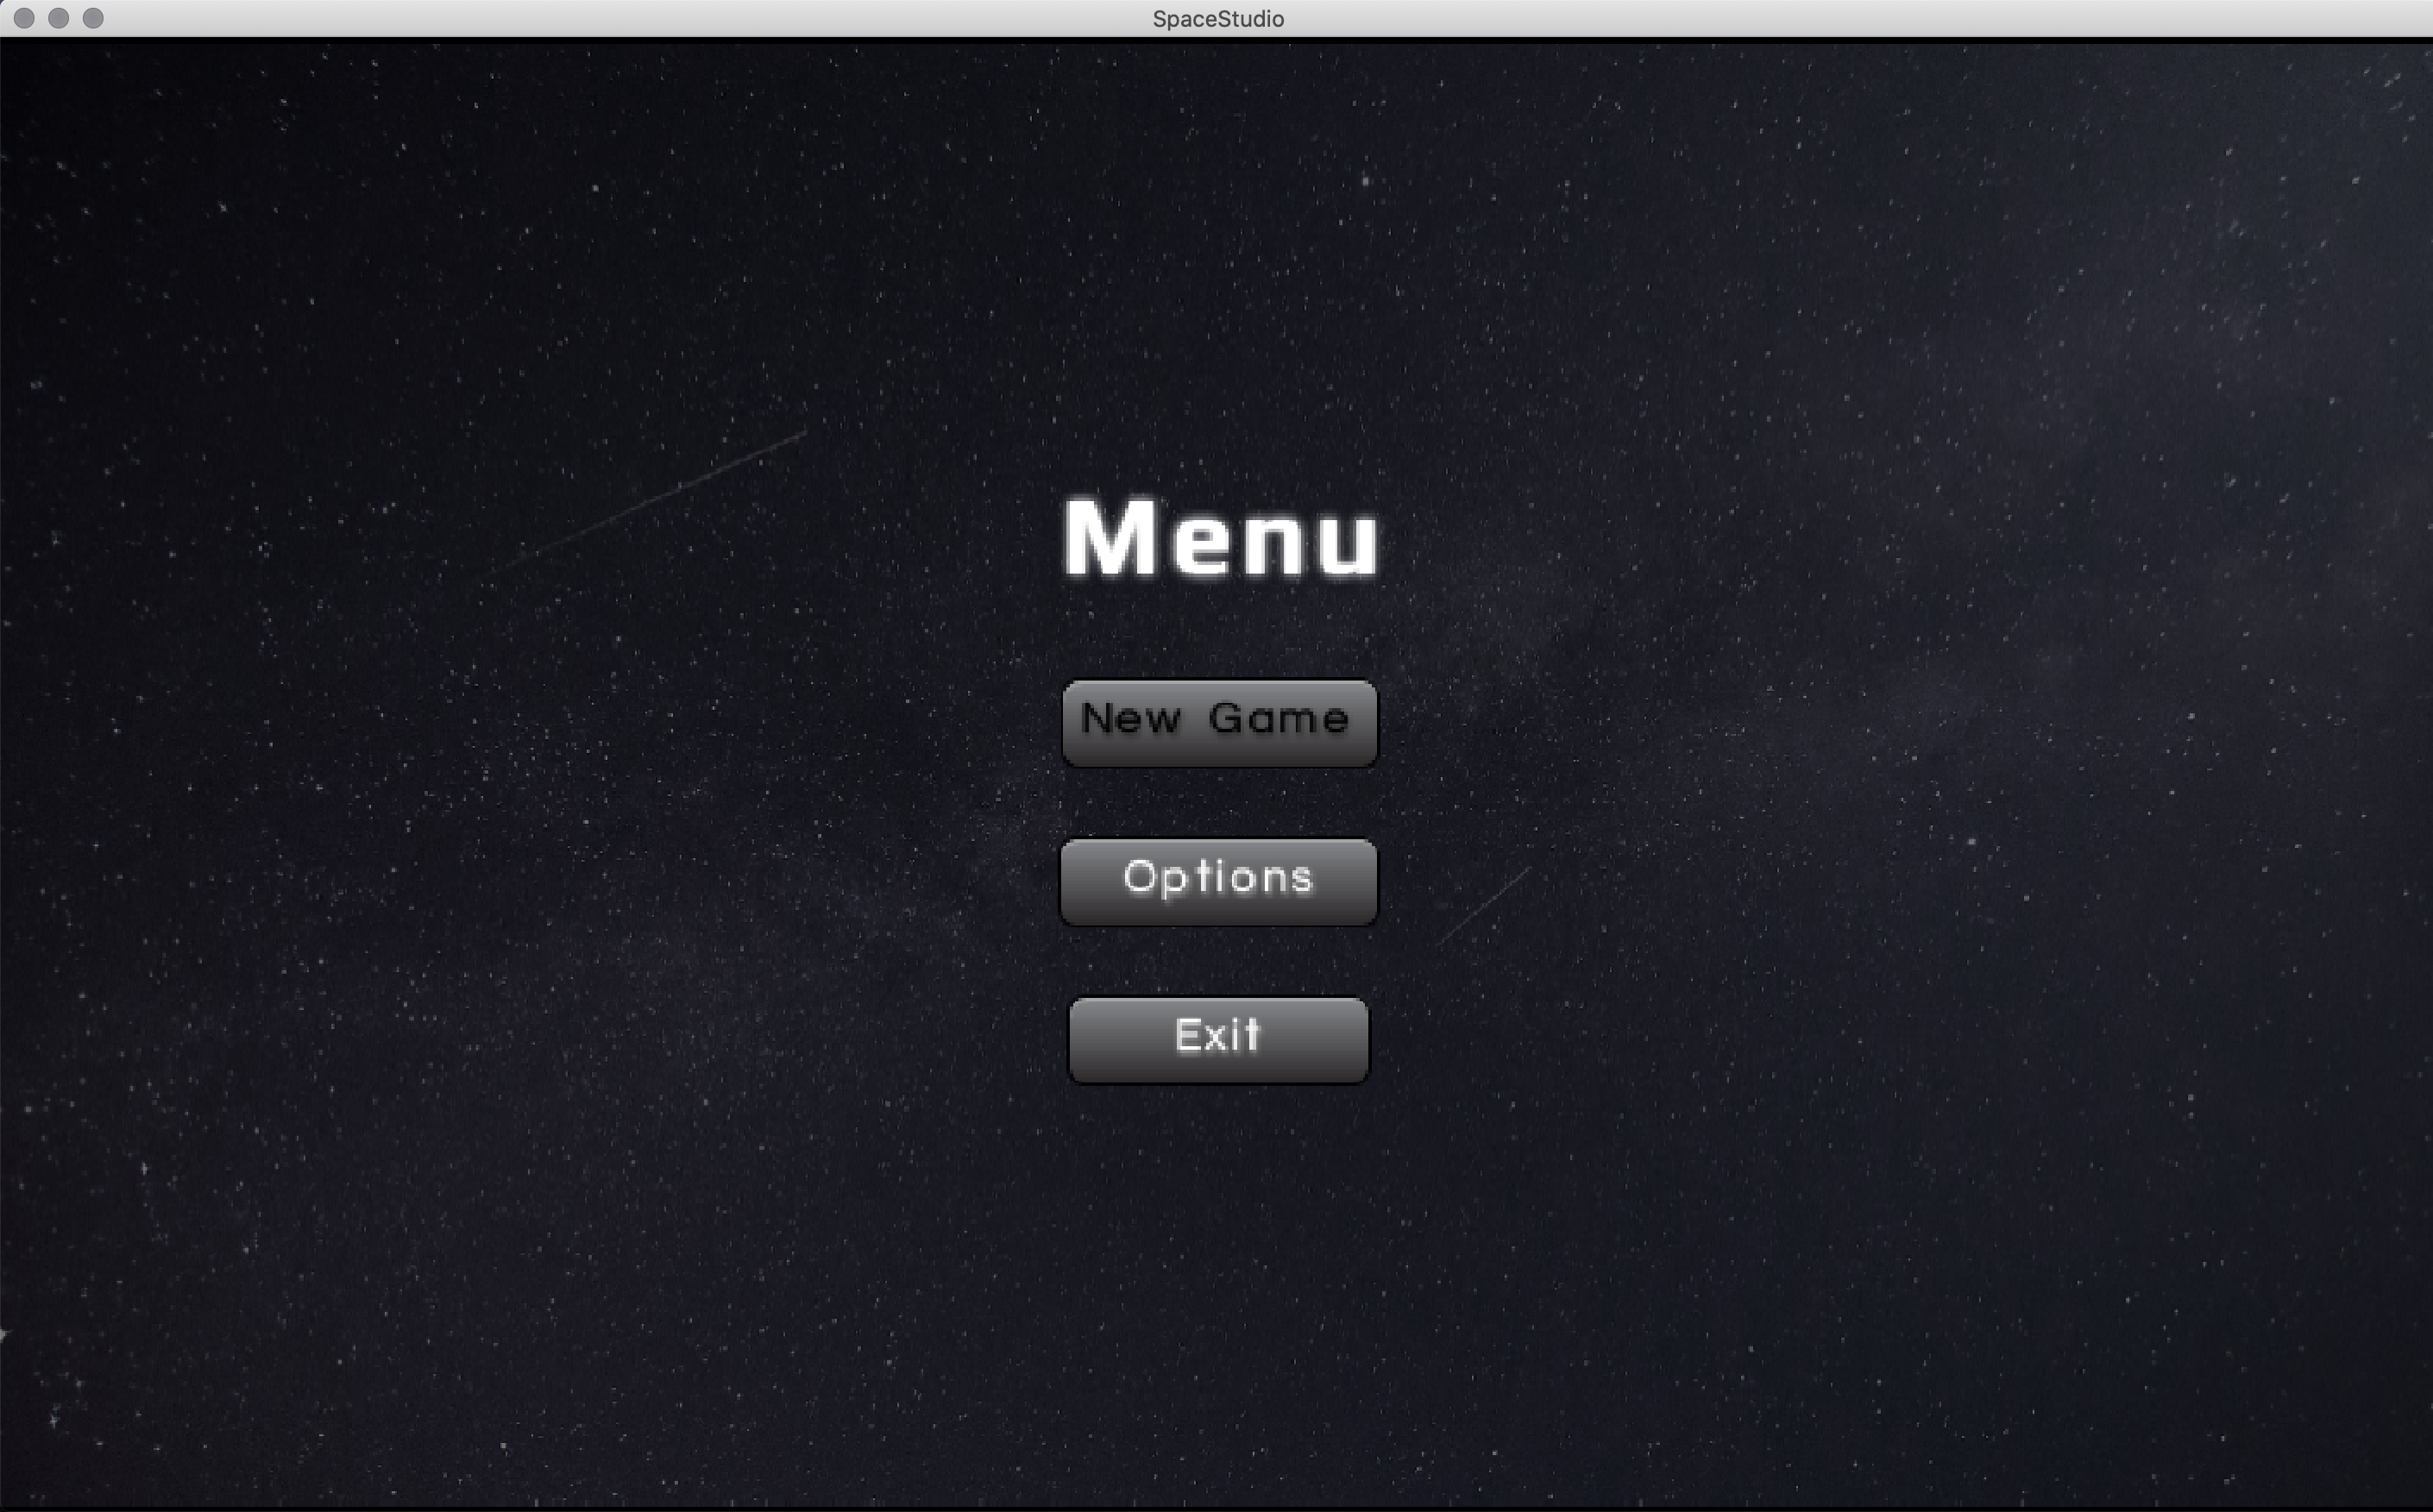
\includegraphics[scale=0.3]{TestProtocolBilder/menuScreen.png}
\caption{Menu Spiel}
\end{figure}
\newpage
\section{Game options}
Im zweiten Menübildschirm können Sie die Optionen sehen, die der Benutzer spielen muss.
\begin{itemize}
\item Single Player: Mit dieser Option kann der Benutzer individuell im Universum spielen.
\item Multiplayer: Diese Option ermöglicht es dem Benutzer, mit einem anderen Spieler im Universum zu spielen und gegeneinander zu kämpfen.
\item Back to Menu: Diese Option ermöglicht es Ihnen, zum vorherigen Bildschirm zurückzukehren.
\end{itemize}
\begin{figure}[h]
\centering
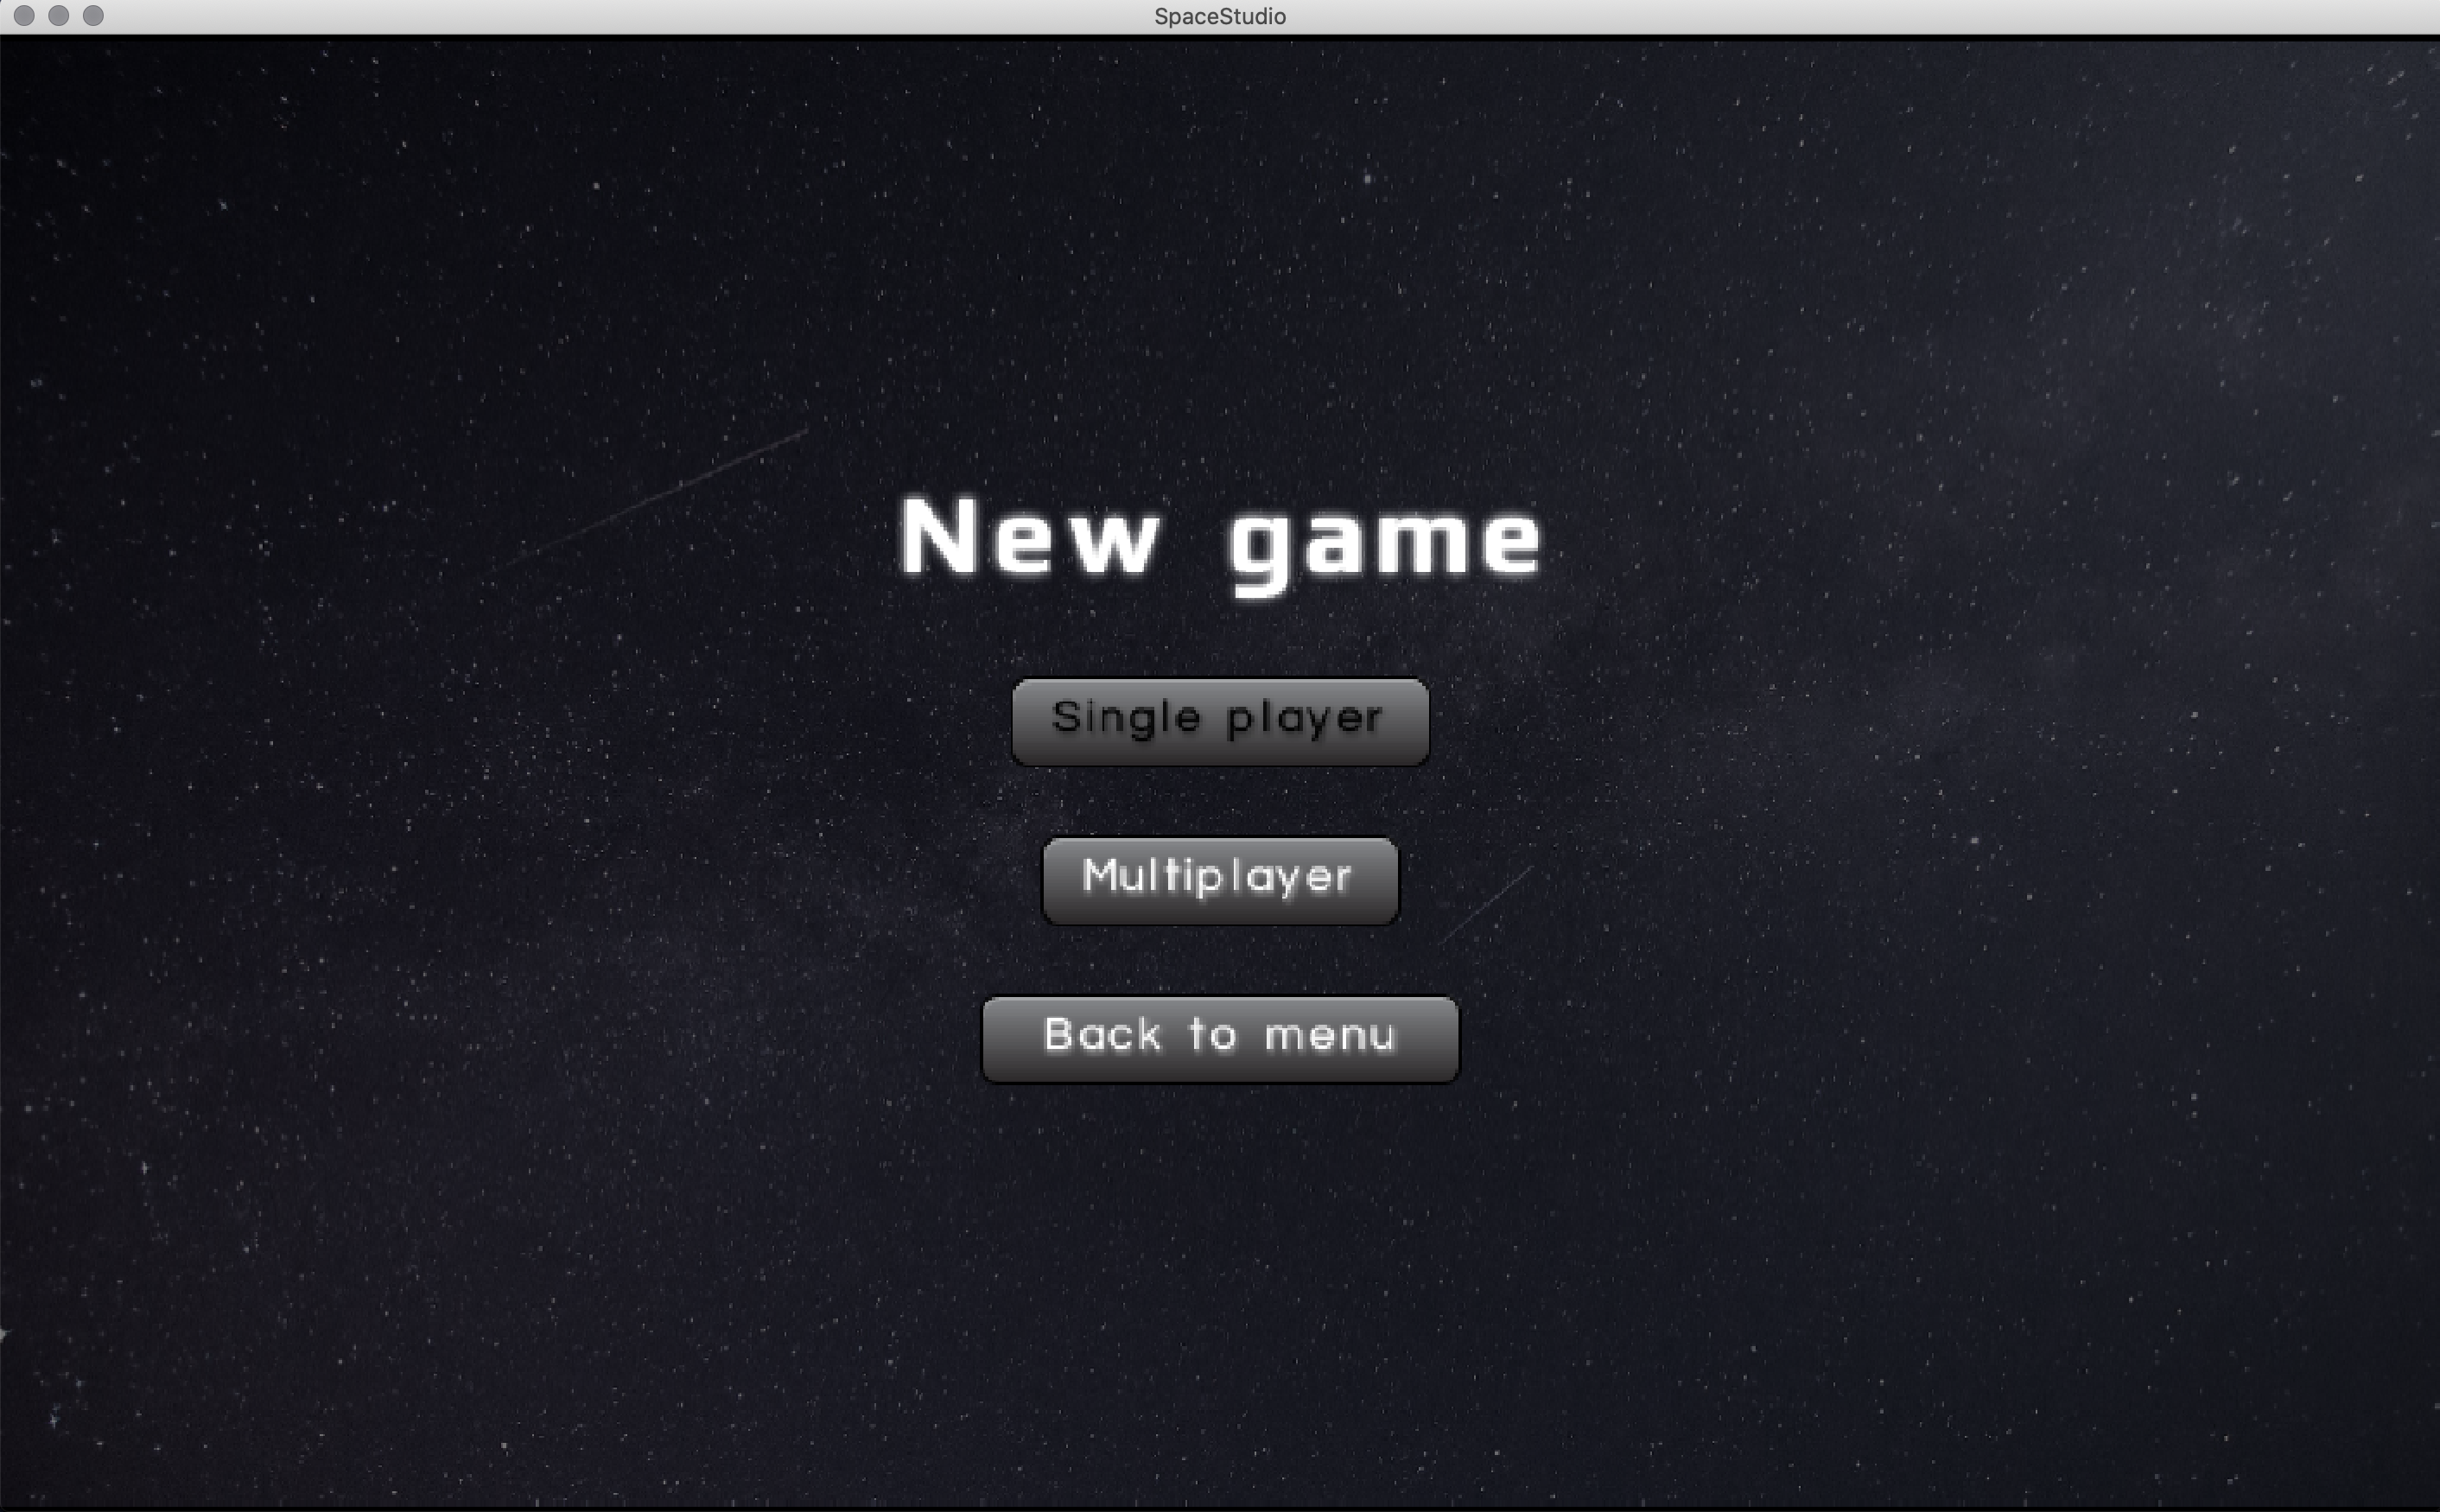
\includegraphics[scale=0.3]{TestProtocolBilder/menuScreenTwo.png}
\caption{Optionen zur Spielen}
\end{figure}
\newpage
\section{Testfall Single Player}
Auf diesem Bildschirm wurde jede Schaltfläche getestet, beginnend mit der Taste Single Palyer.\\
\begin{figure}[h]
\centering
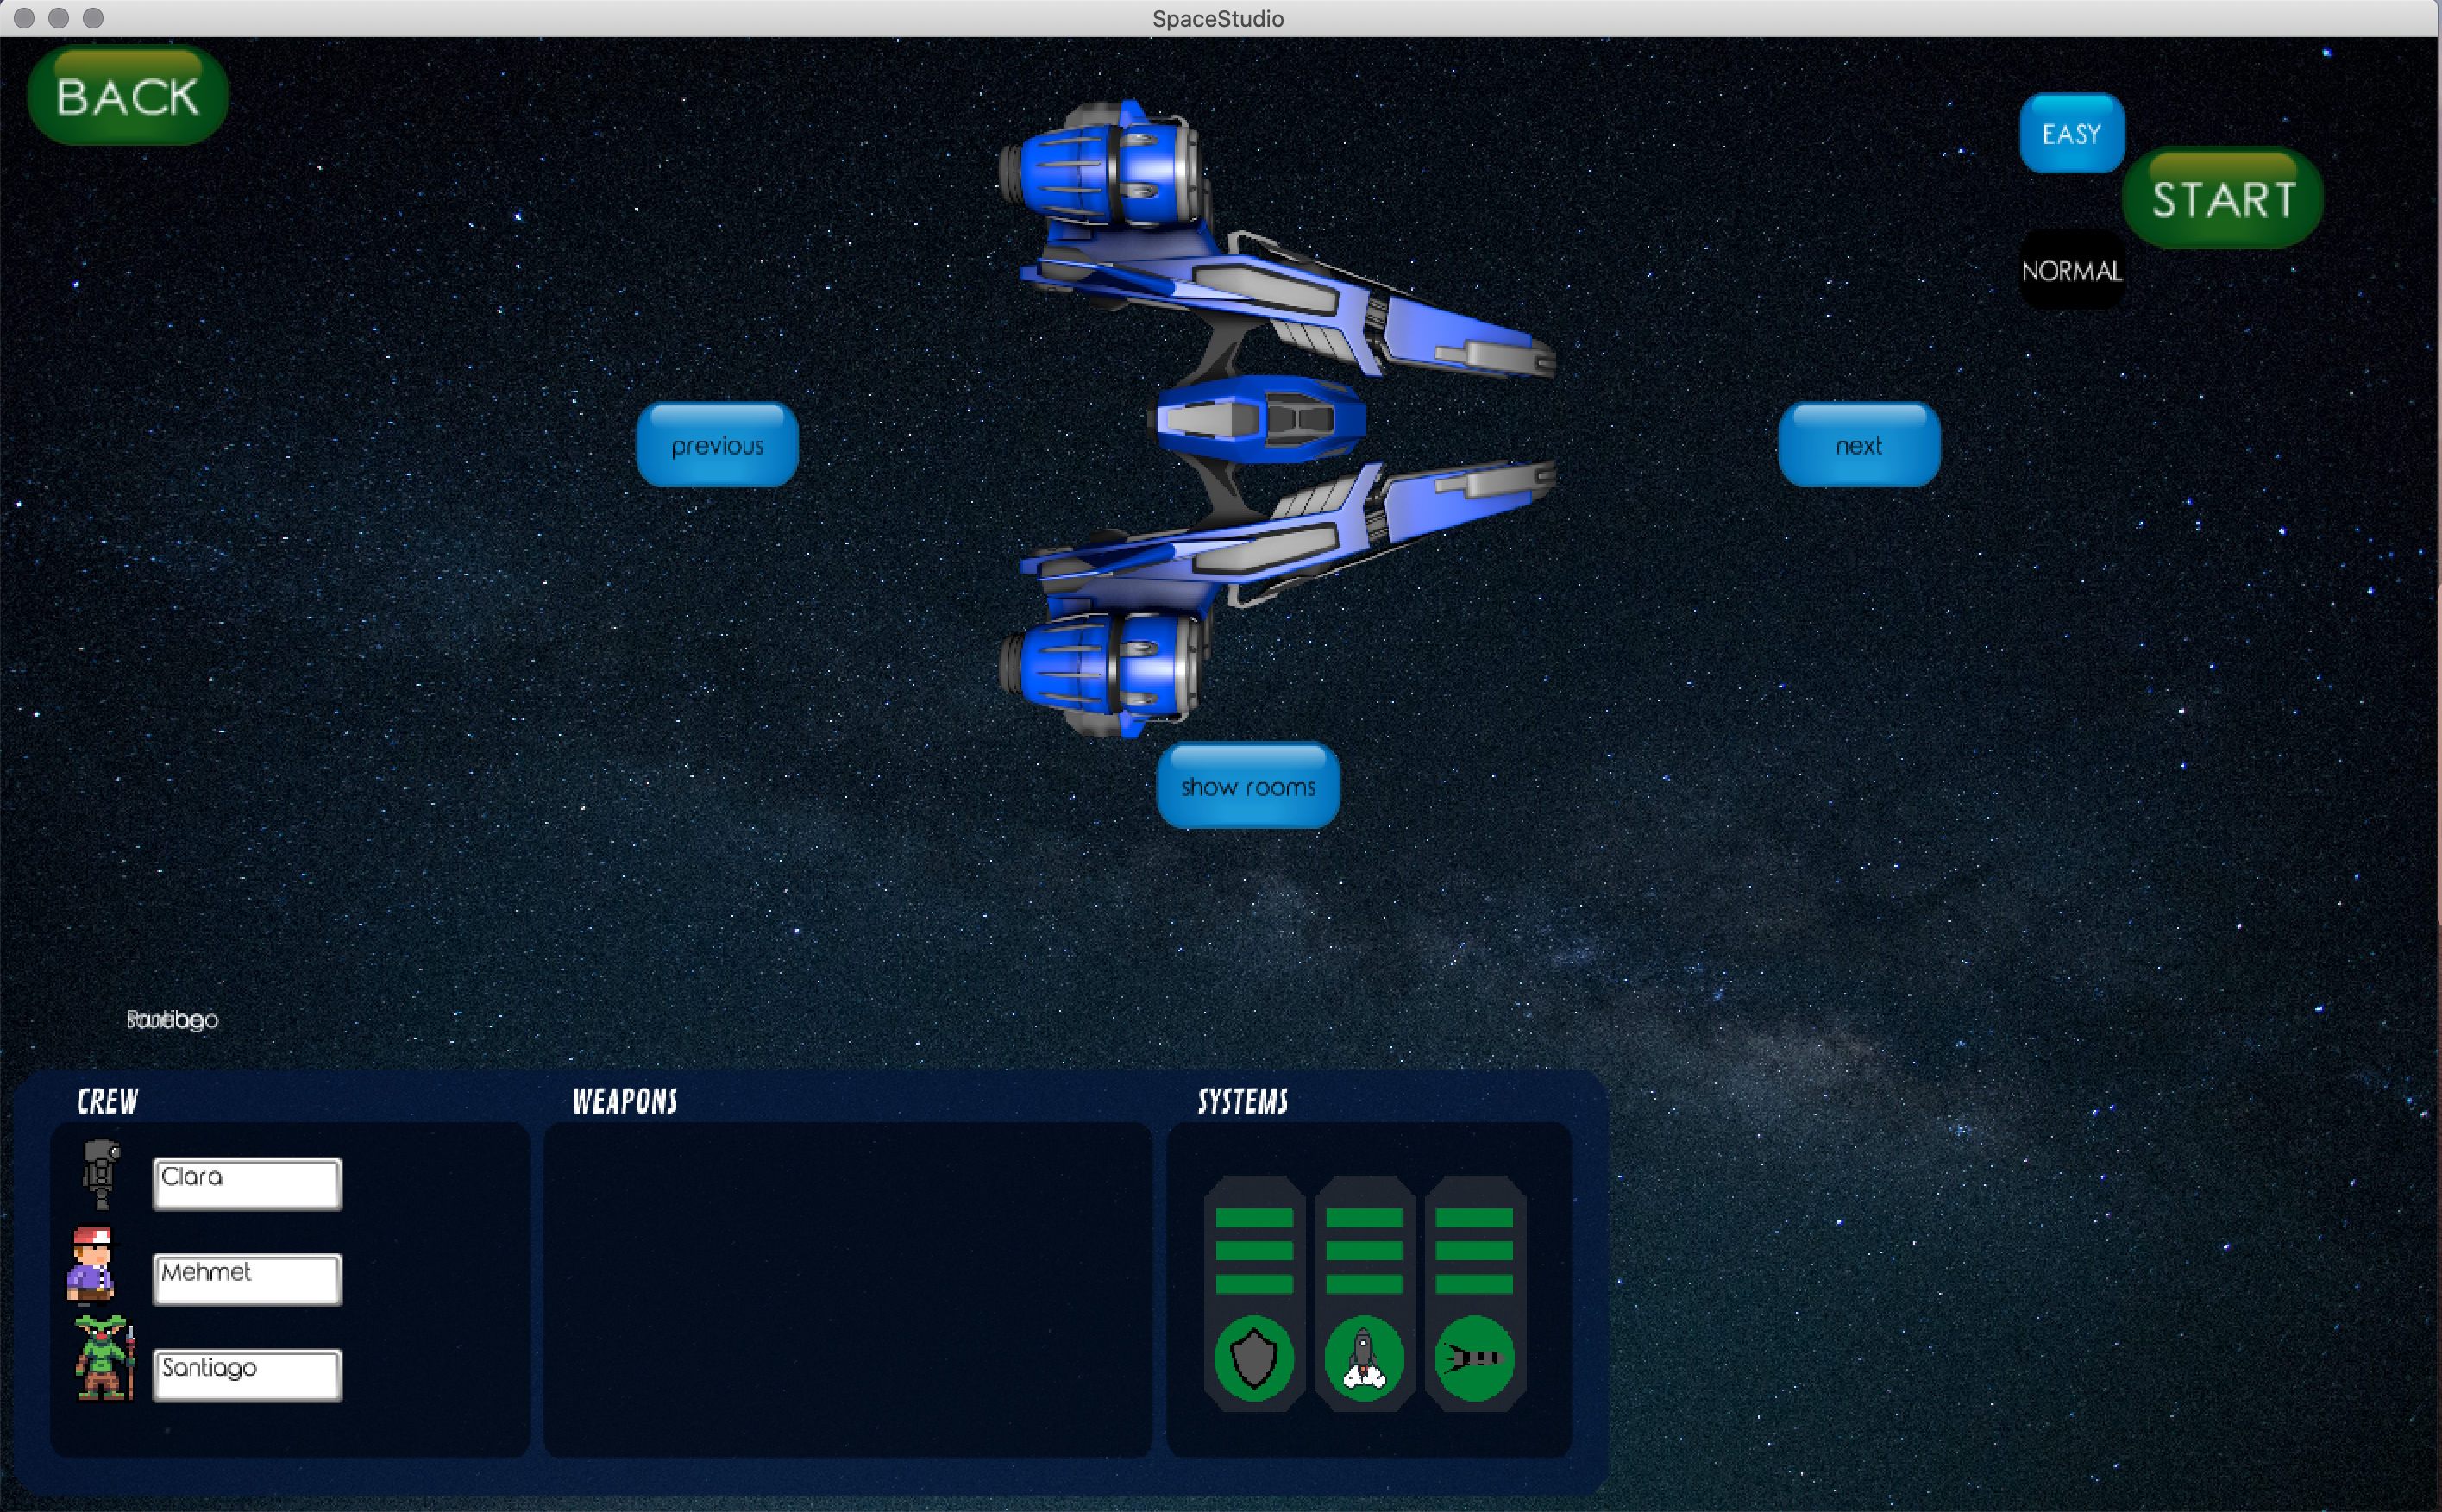
\includegraphics[scale=0.3]{TestProtocolBilder/selecShipScreen.png}
\caption{Select Ship screen}
\end{figure}
\newpage
\subsection{rooms test}

Mit dieser Taste wurde getestet, ob die Abschnitte des Bootes sichtbar sind. Wenn Sie erneut drücken, verschwinden die Abschnitte\\
\begin{figure}
\centering
\includegraphics[scale=0.3]{TestProtocolBilder/shipRooms.png}
\caption{romms of the ship}
\end{figure}

\newpage
\subsection{andere Ships}
Mit der nächsten Schaltfläche kann der Benutzer die möglichen Schiffe für das Spiel sehen
\begin{figure}
\centering
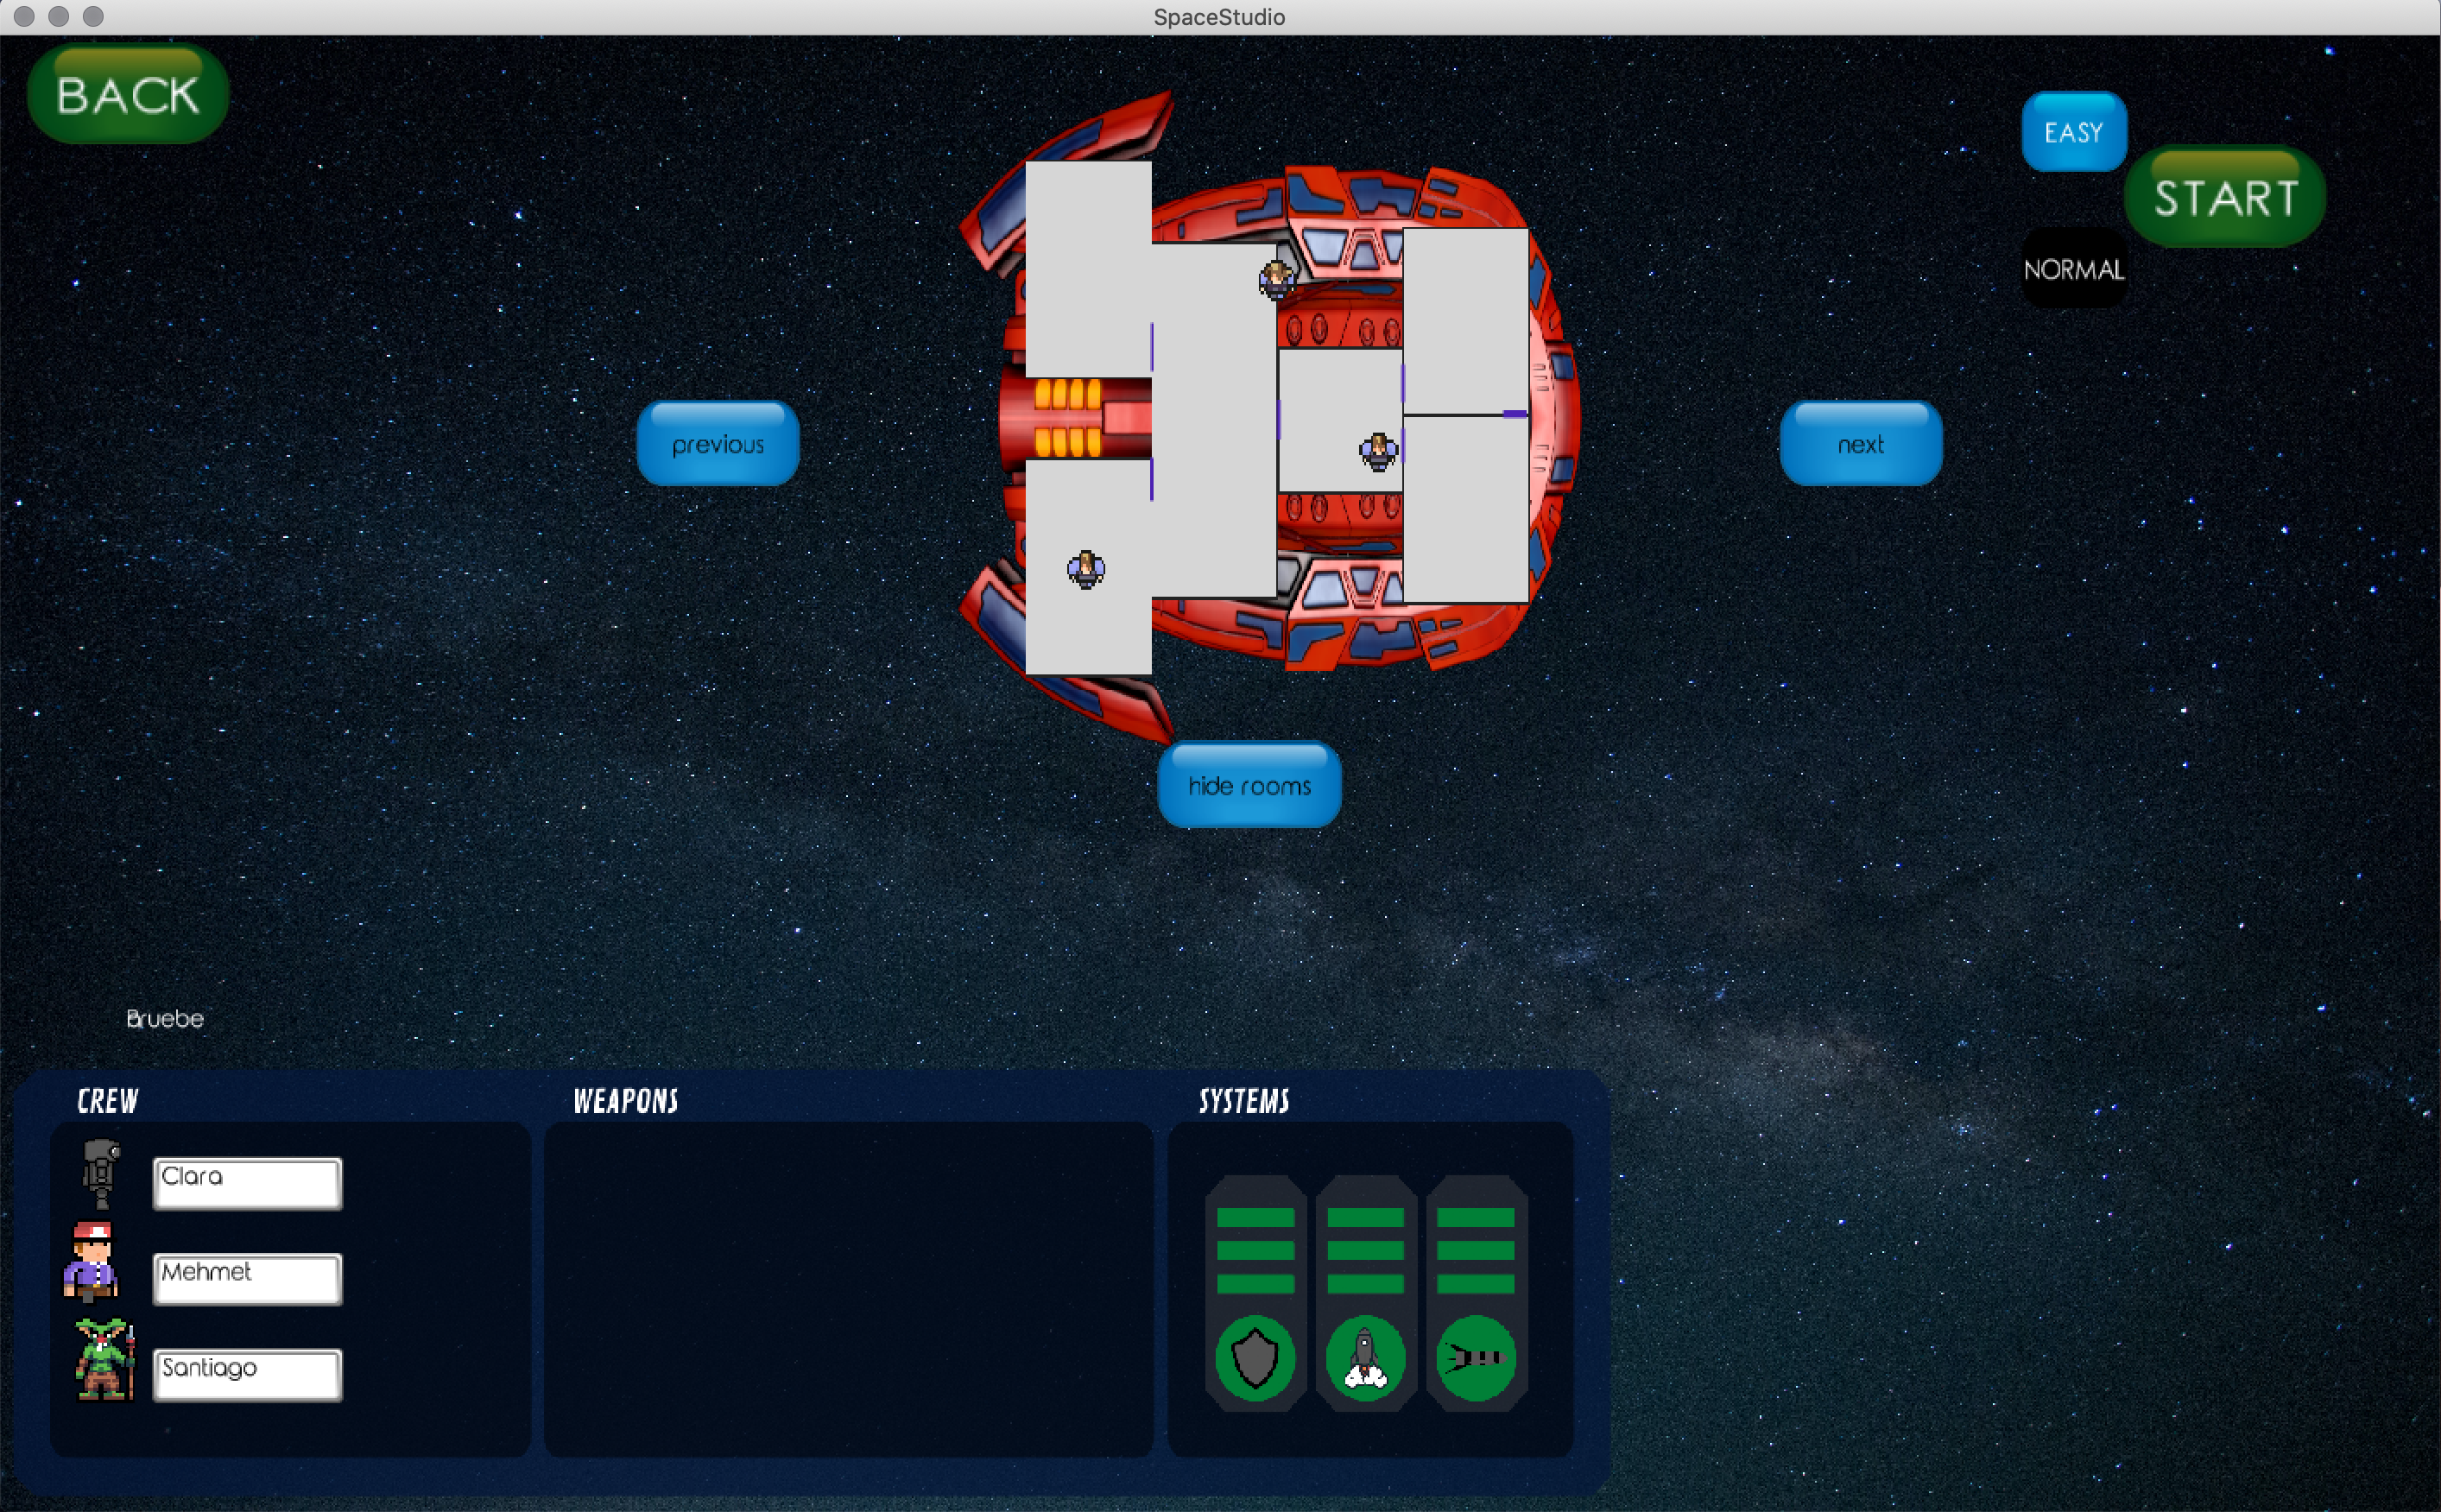
\includegraphics[scale=0.3]{TestProtocolBilder/next.png}
\caption{posible other ships}
\end{figure}

\newpage
\subsection{Universe Schwierigkeit}

Diese Testschaltfläche ermöglicht die Schaffung eines größeren Universums, in dem es mehr Planeten mit unterschiedlichen Eigenschaften gibt\\
\begin{figure}
\centering
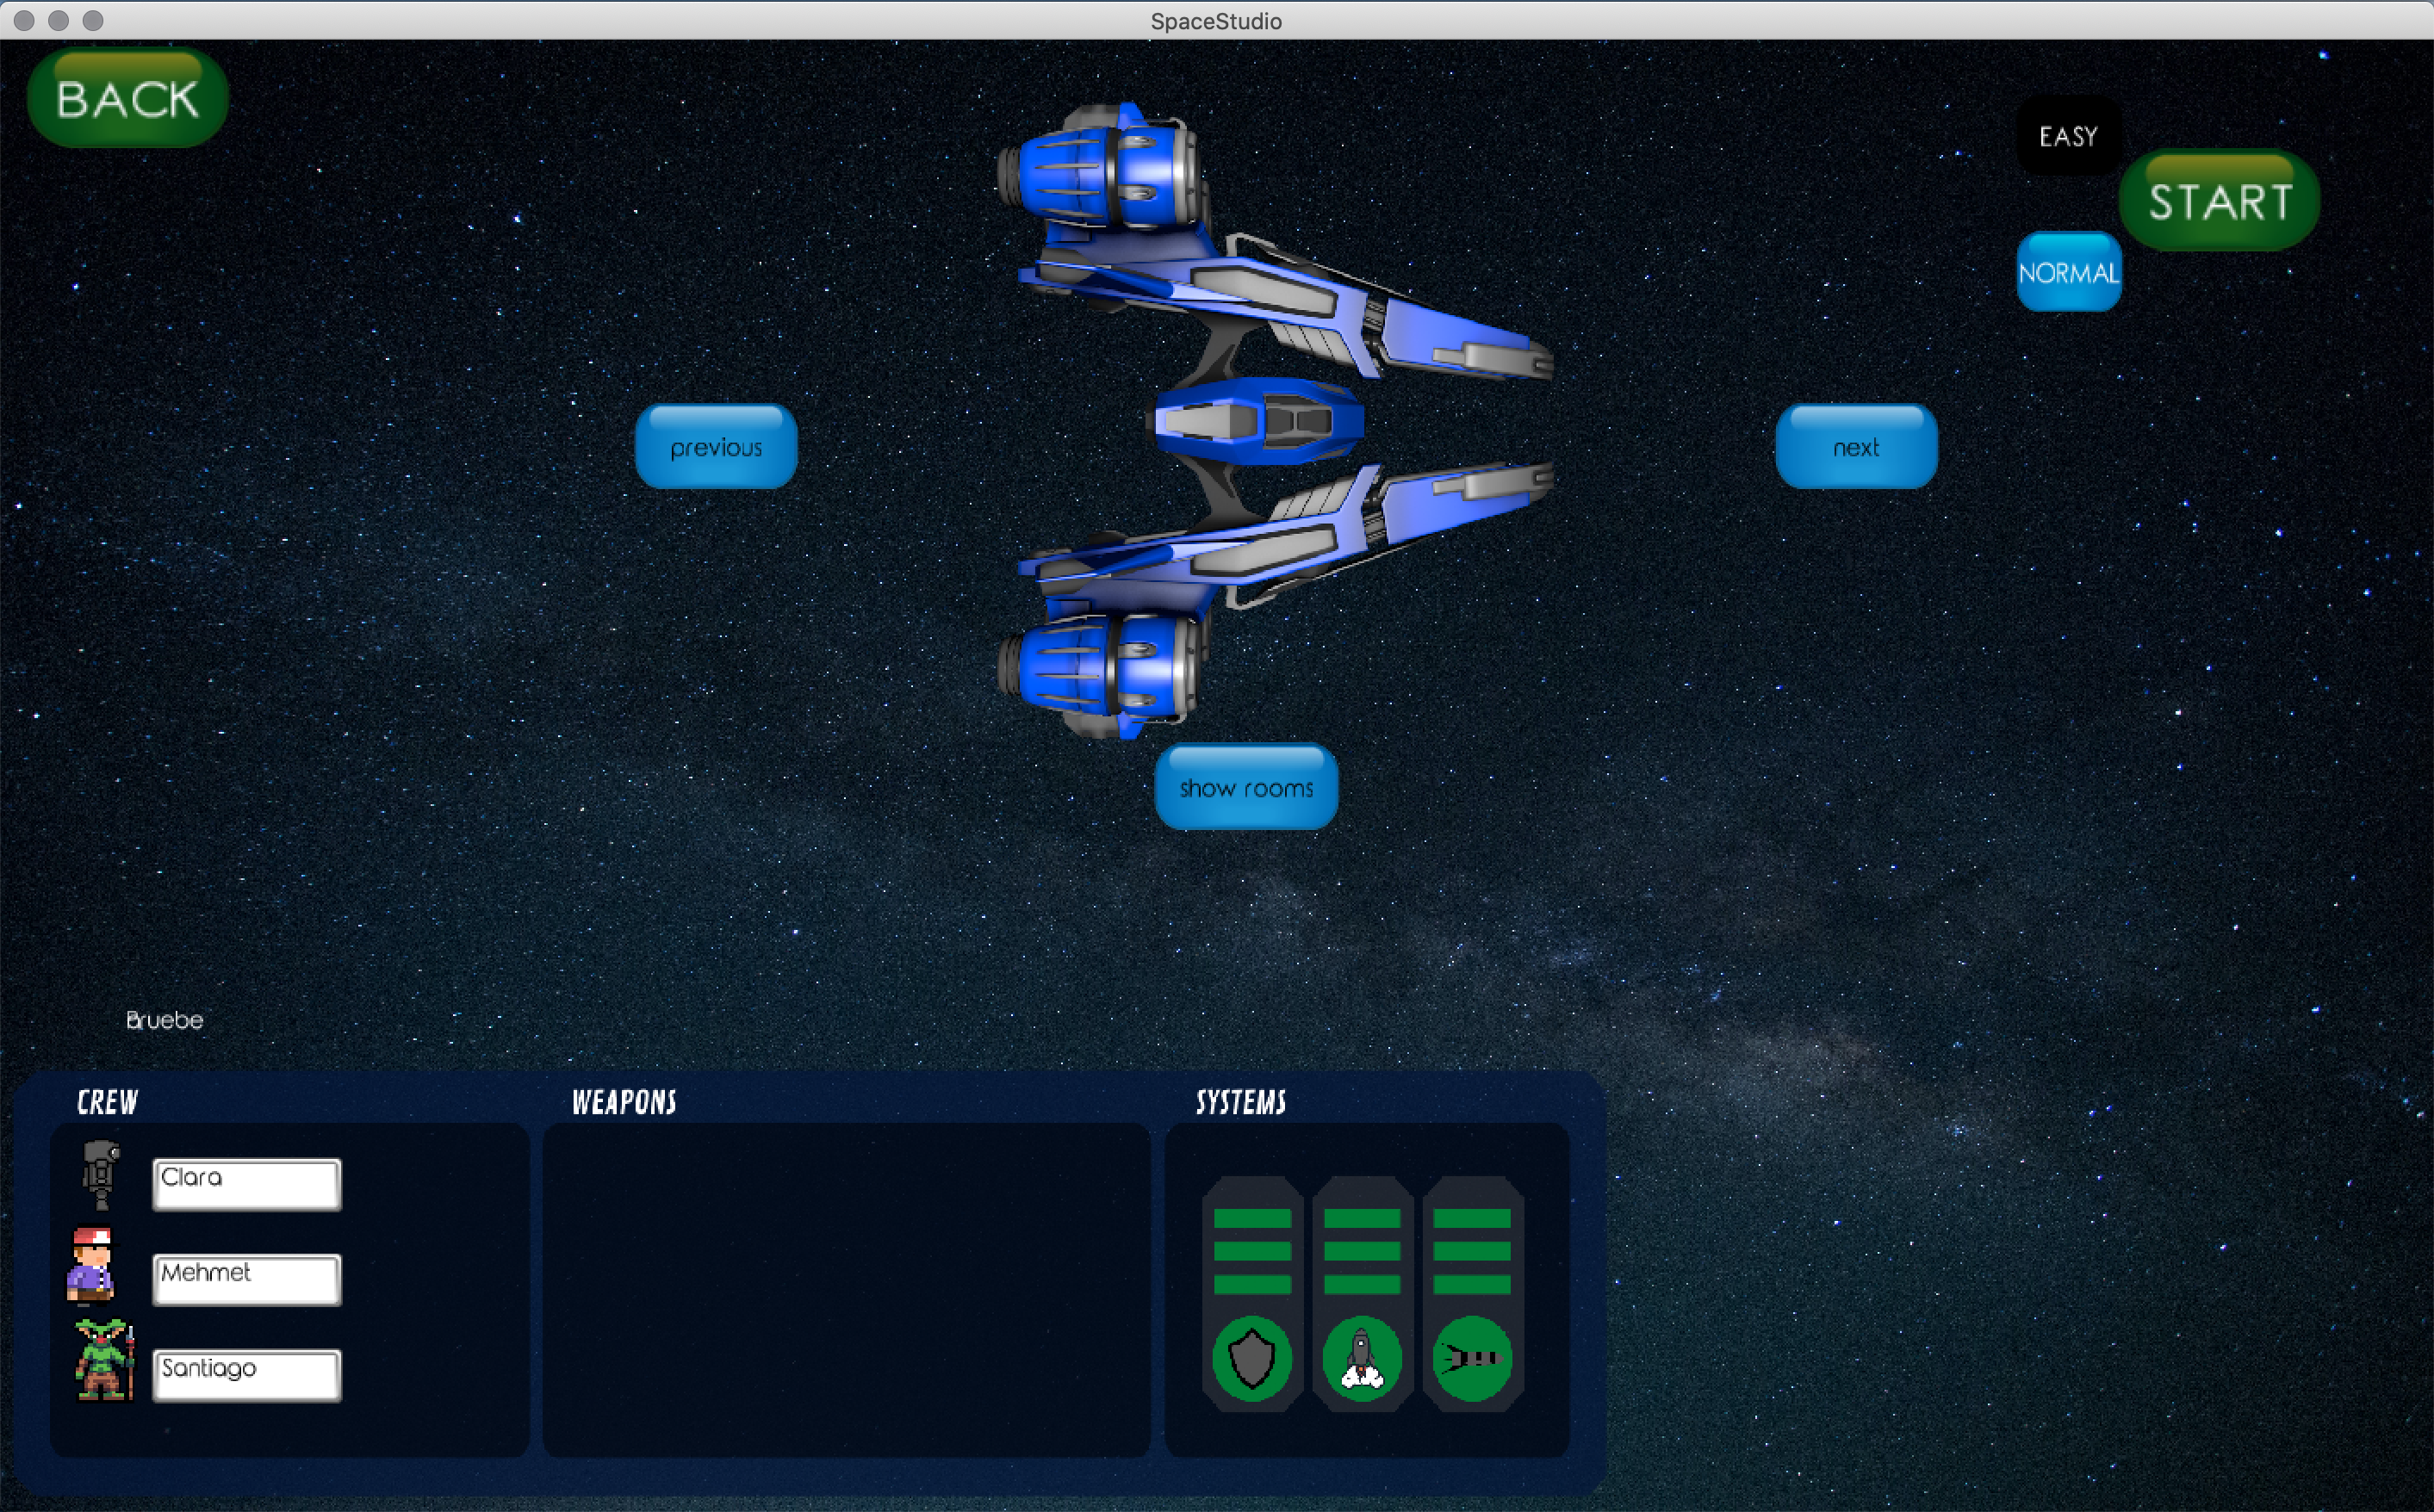
\includegraphics[scale=0.3]{TestProtocolBilder/universeButon.png}
\caption{easy and normal mode}
\end{figure}

\newpage
Das Universum mit einer komplexeren Schwierigkeit wird korrekt erstellt.\\

\begin{figure}[t]
\centering
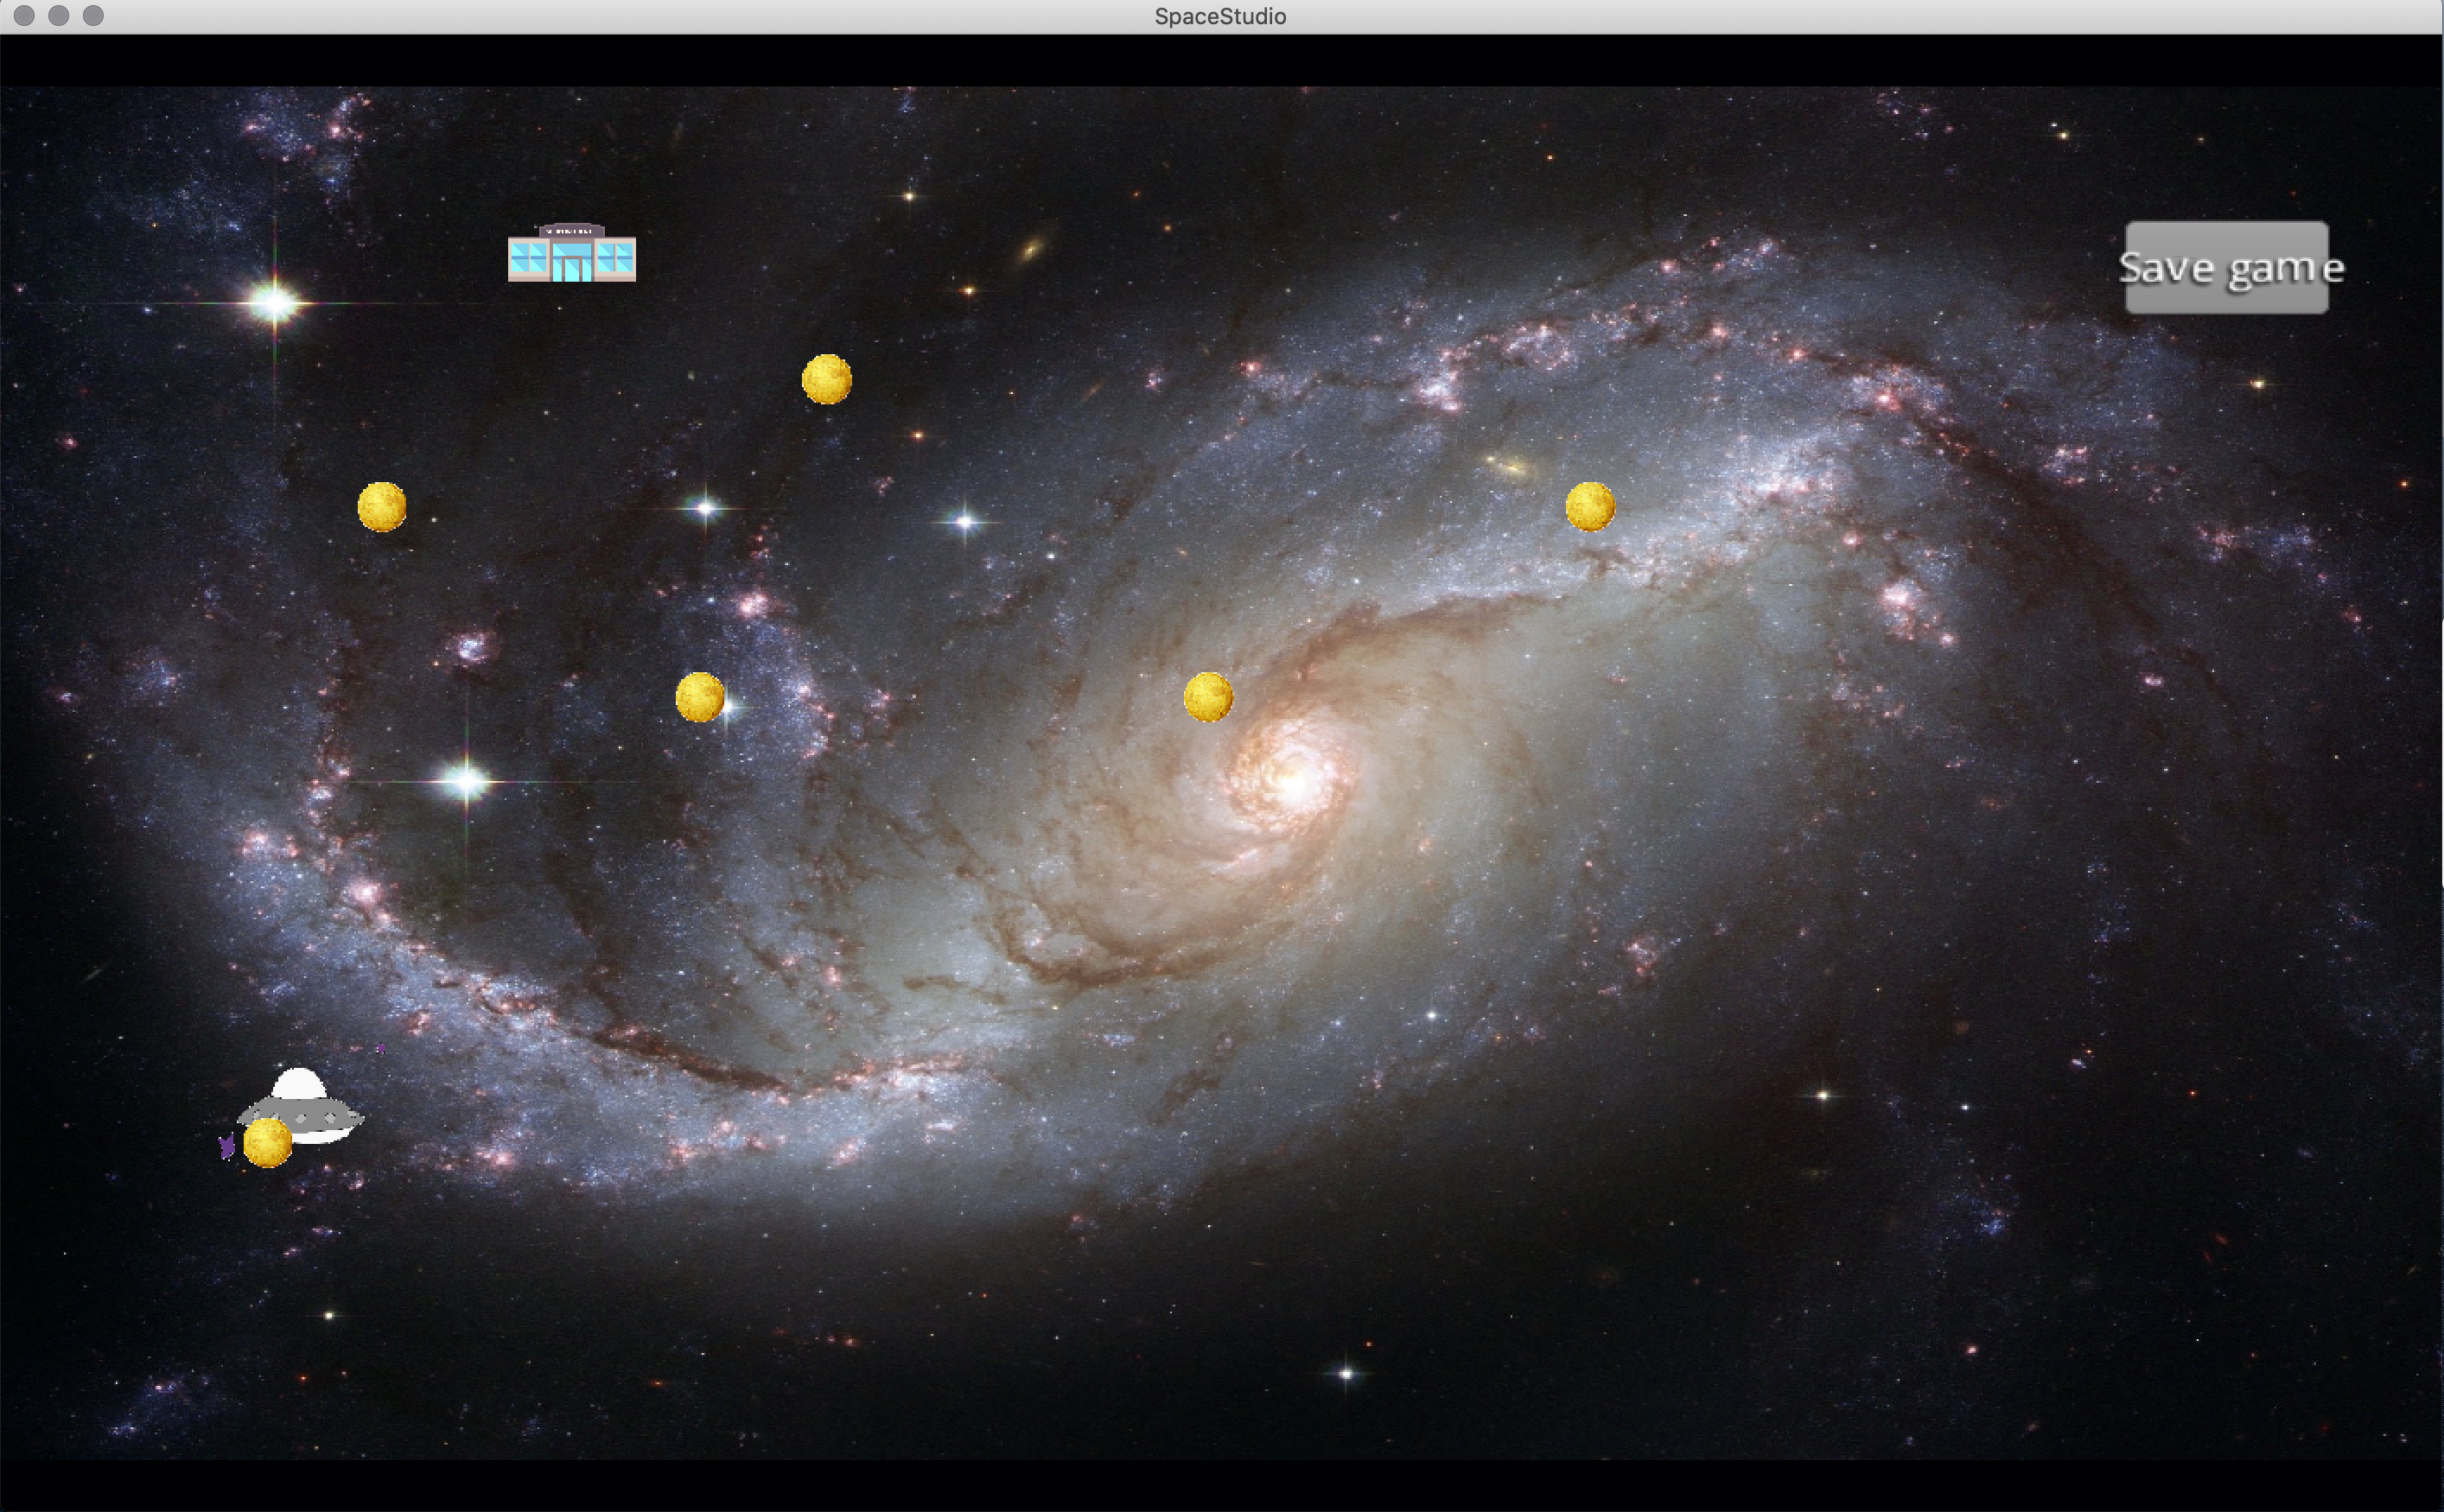
\includegraphics[scale=0.3]{TestProtocolBilder/universeHard.png}
\caption{universe normal mode}
\end{figure}

Die Schaltfläche, die das Beenden des Universums erleichtert, wurde ebenfalls getestet.\\

\begin{figure}[t]
\centering
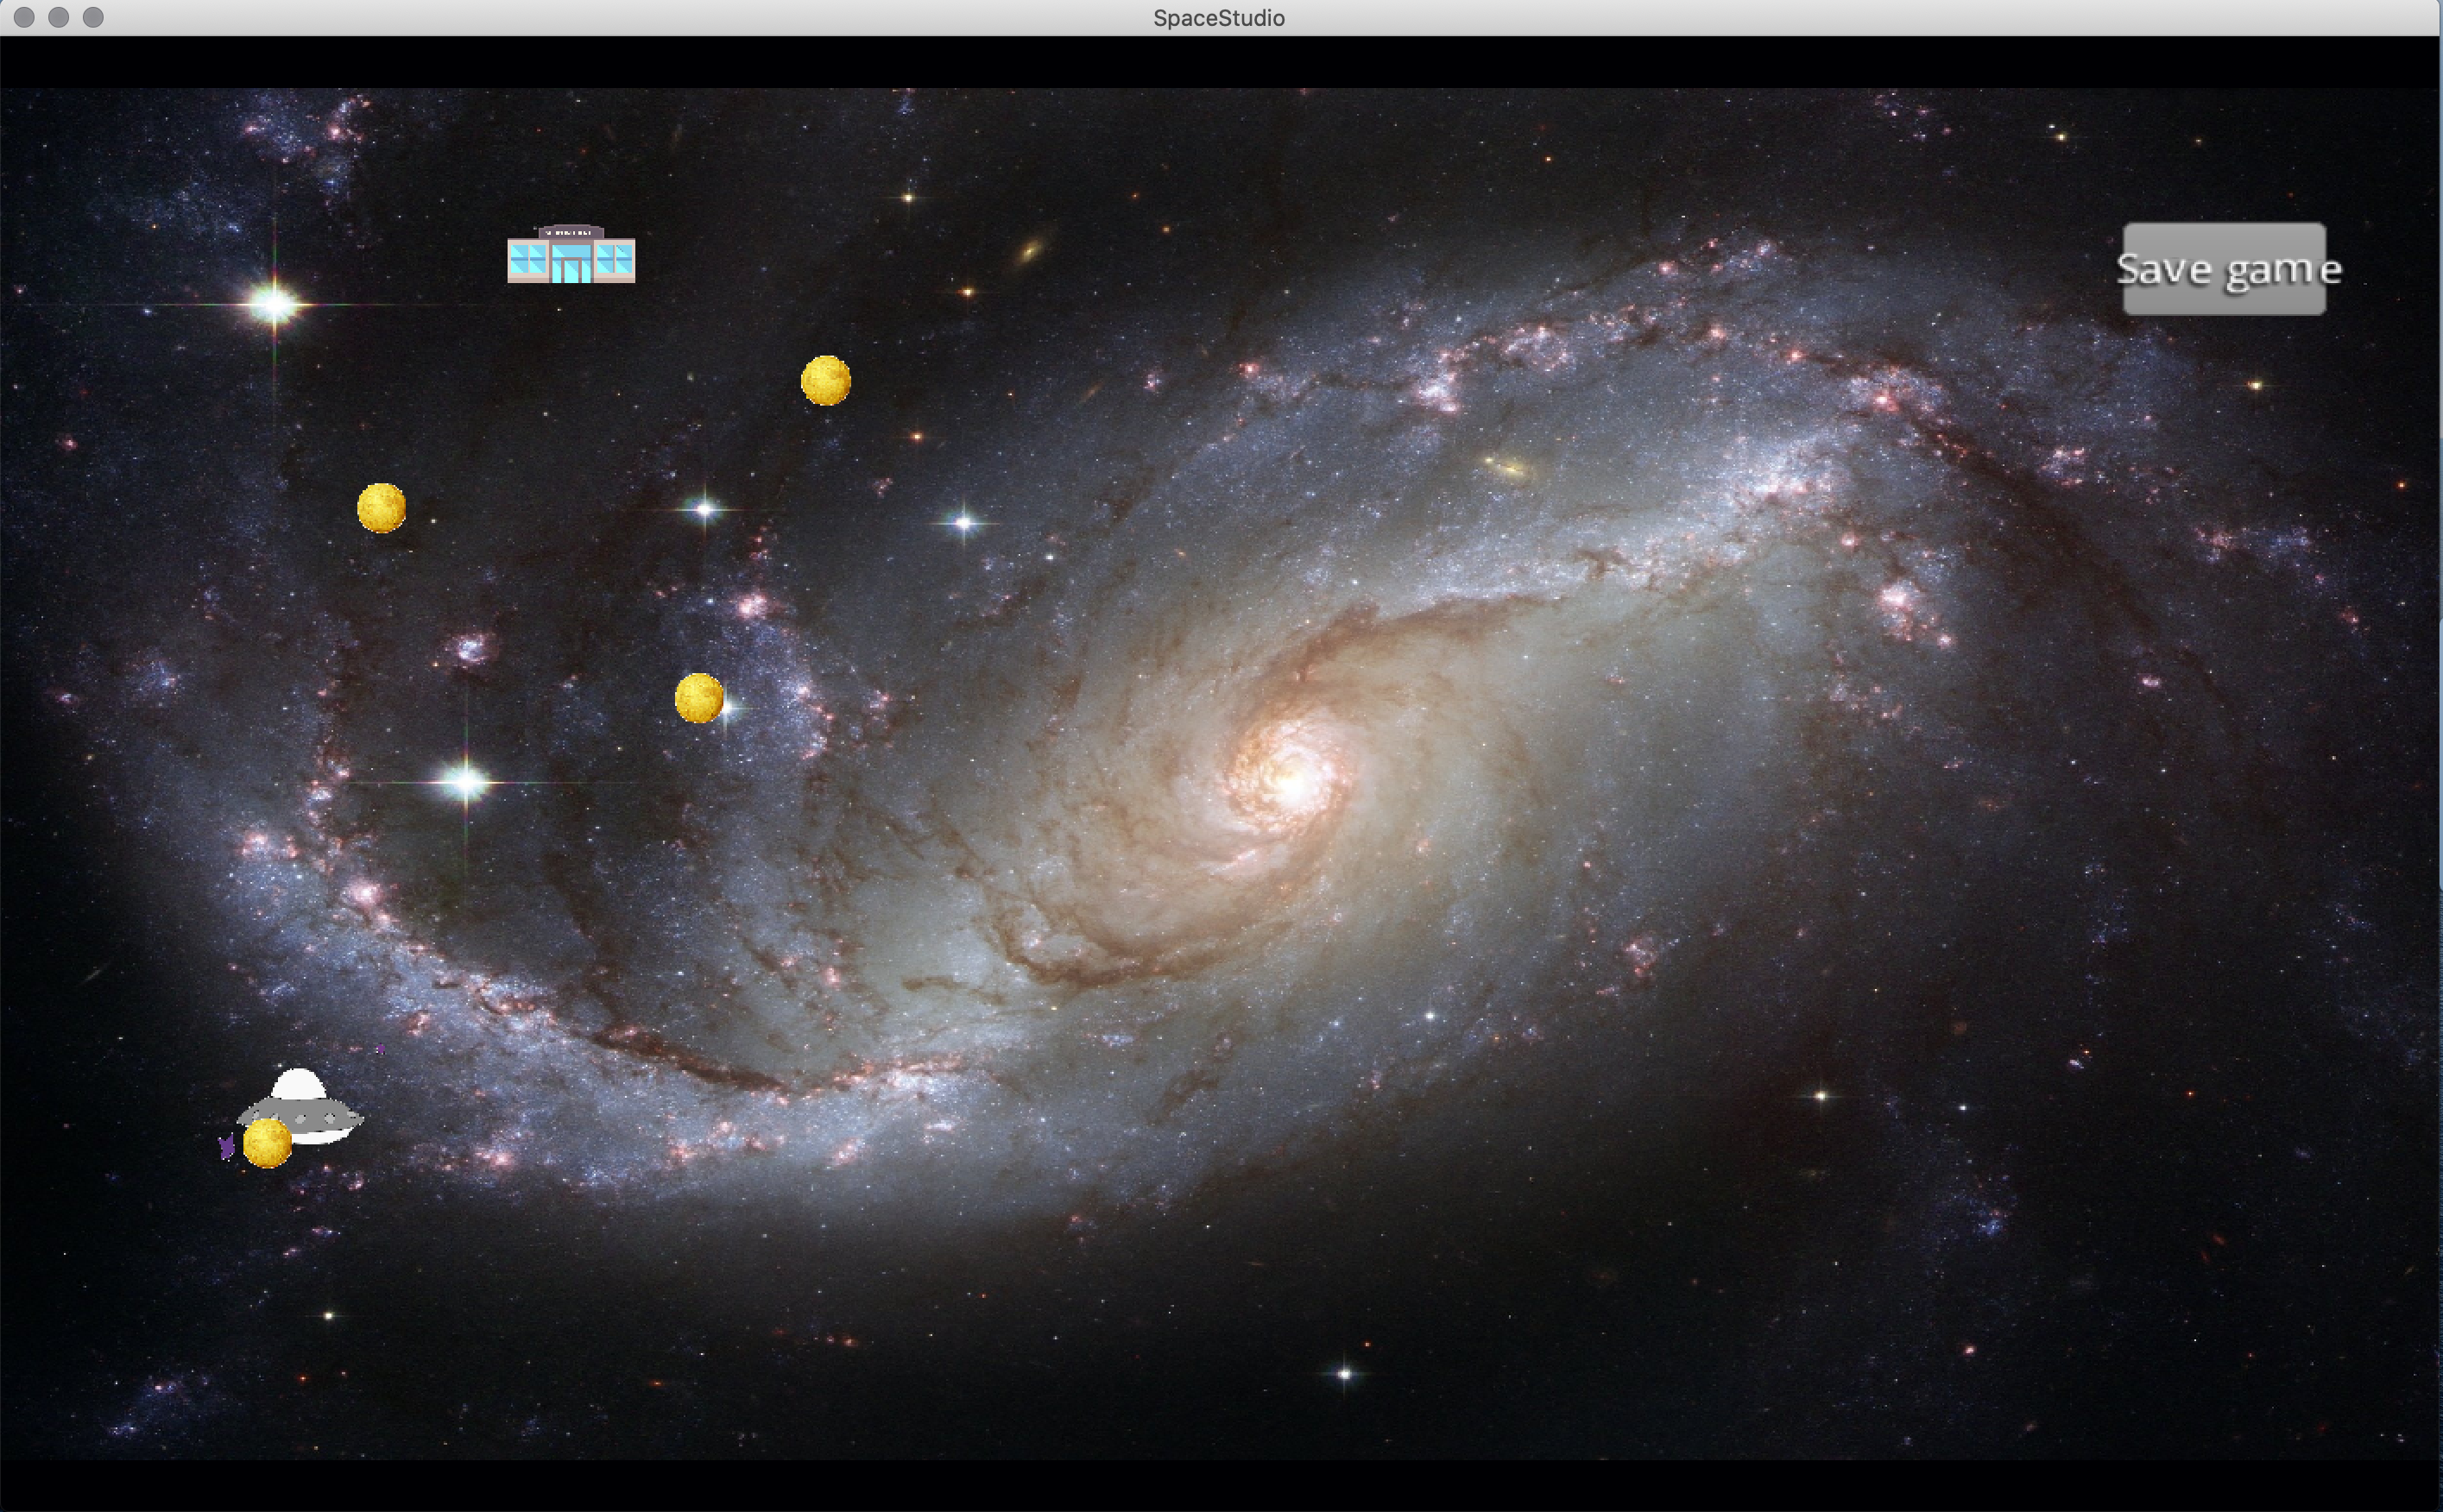
\includegraphics[scale=0.3]{TestProtocolBilder/universeEase.png}
\caption{universe in ease mode}
\end{figure}

\newpage
\subsection{Map}

Hier wurden jeder Planet und jede Station getestet, die Schaltflächen sind und den Zugang zum Geeignise-Bildschirm ermöglichen.\\
\begin{figure}
\centering
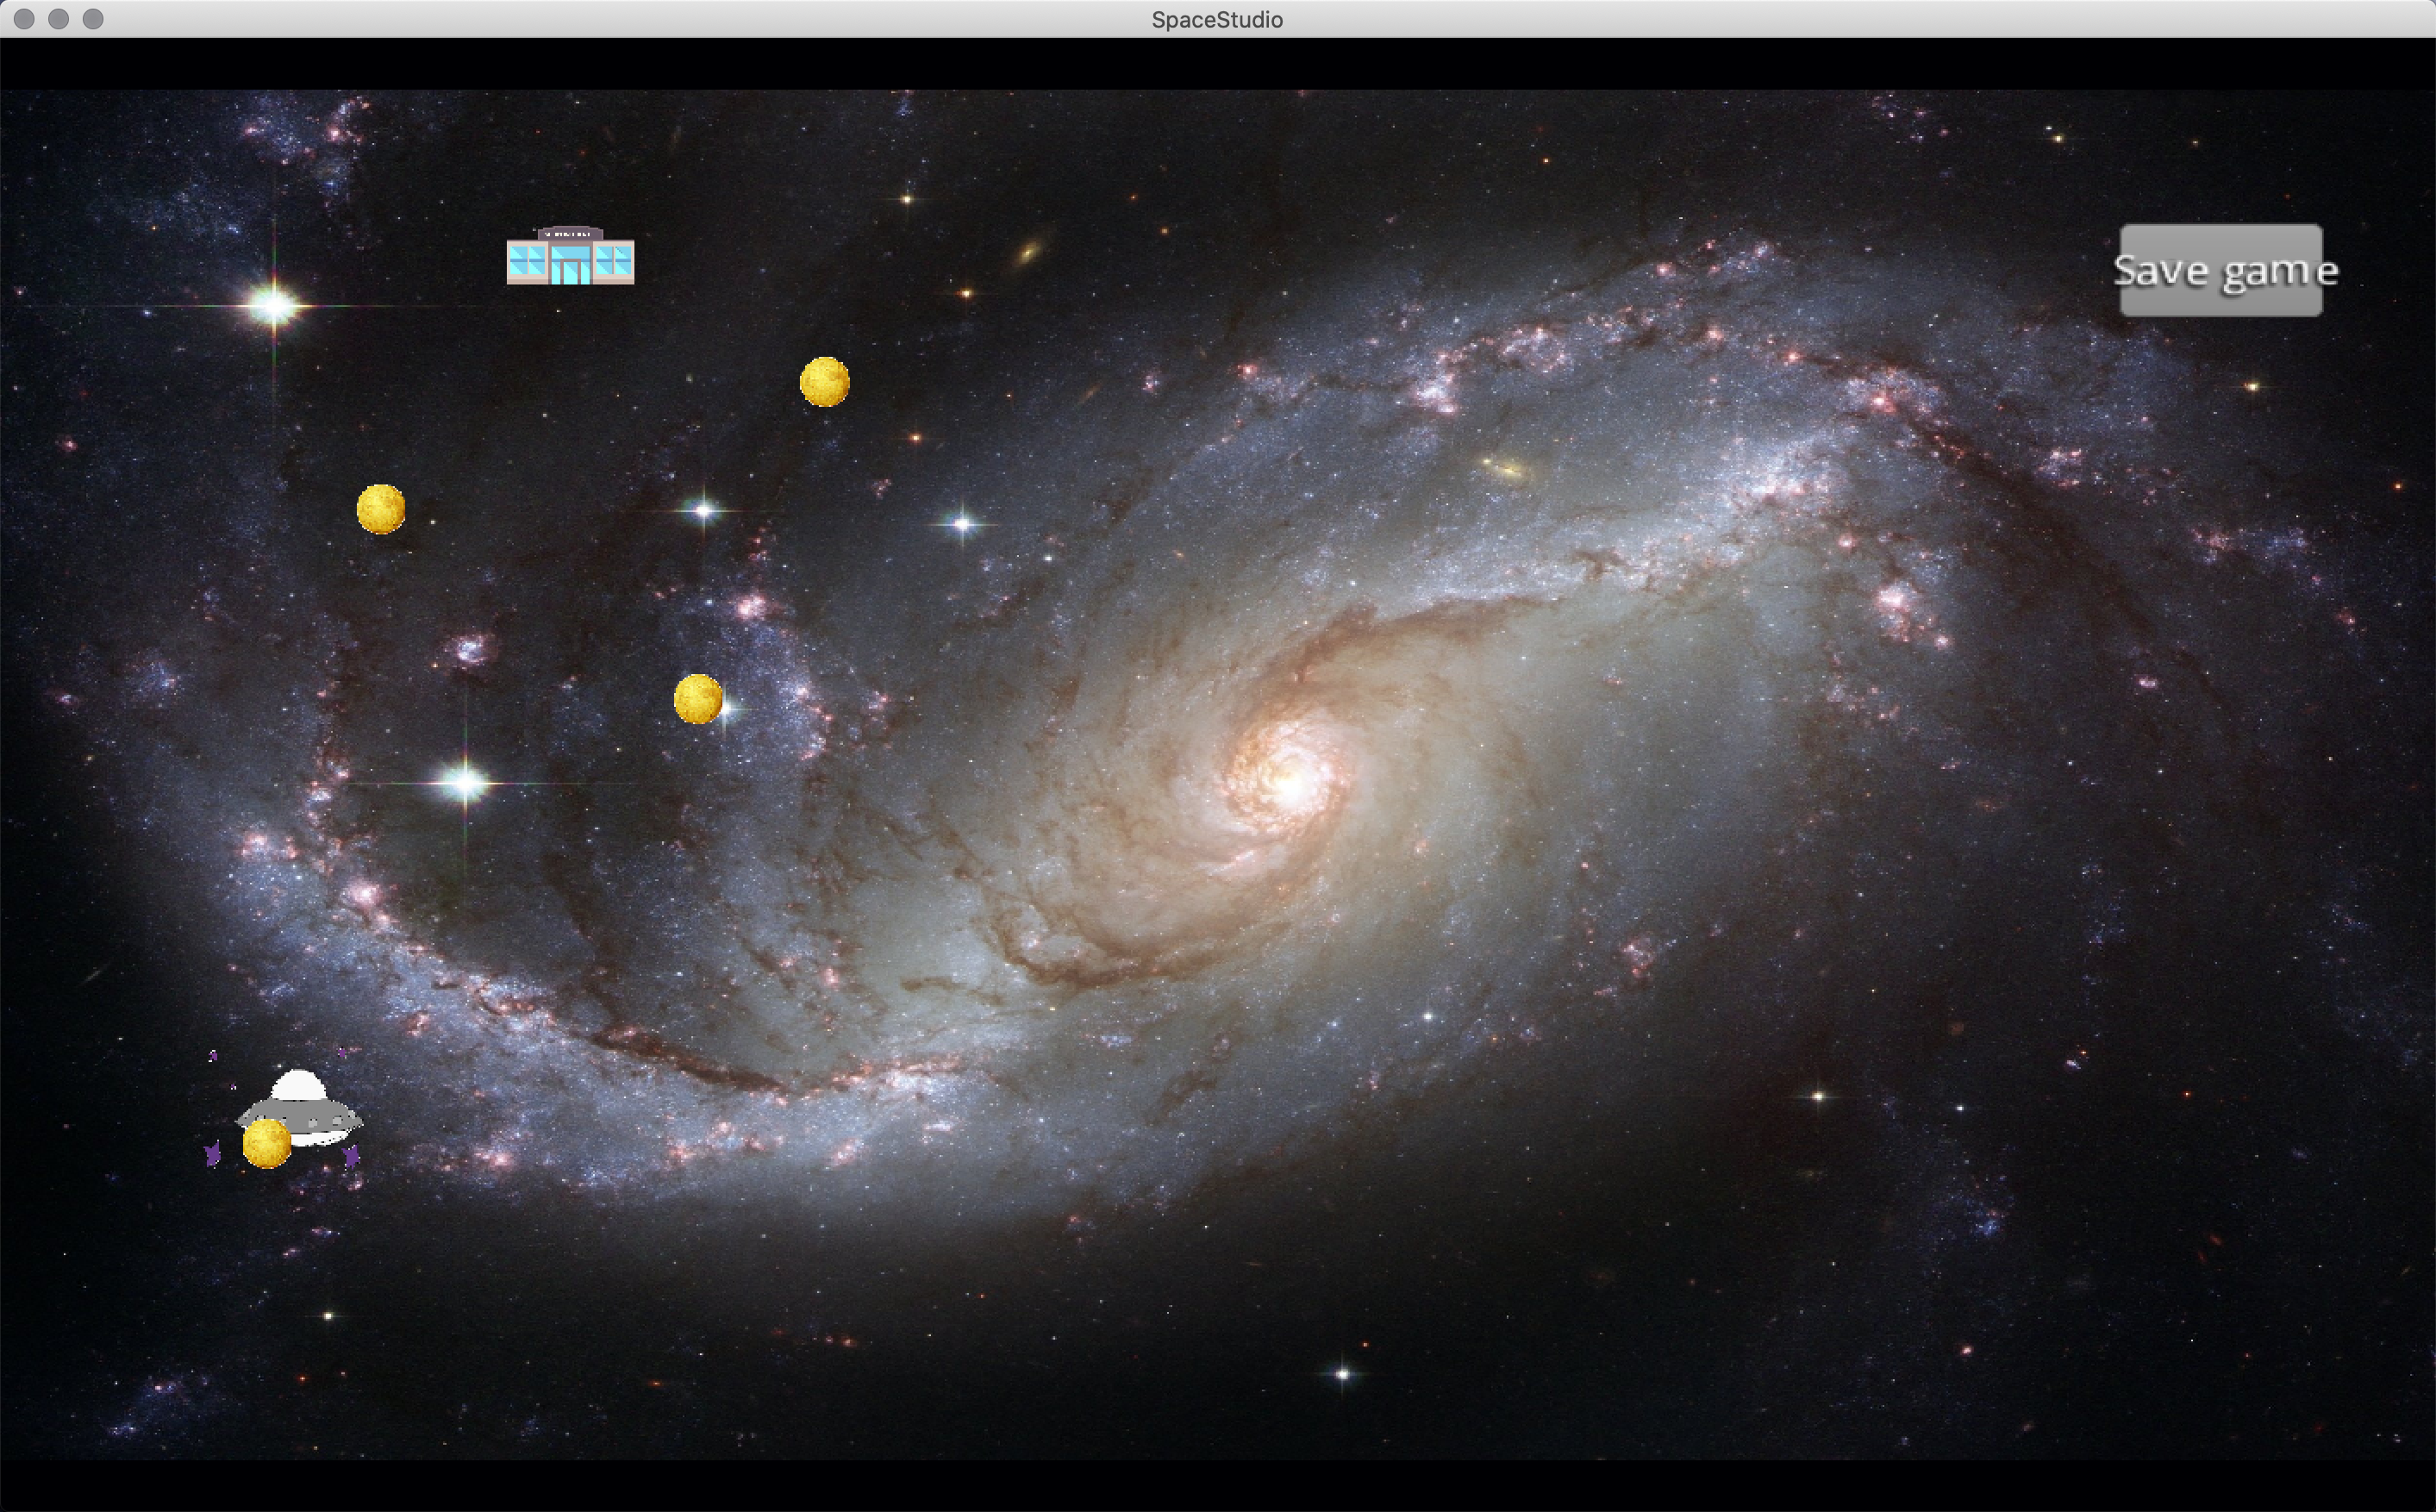
\includegraphics[scale=0.3]{TestProtocolBilder/map.png}
\caption{Game Map}
\end{figure}
\newpage
\section{Geeingnissen}
Nach dem Drücken eines Planeten wird ein PopUp-Menü angezeigt und die Sprungfunktion getestet.
\begin{figure}[htp]
\centering
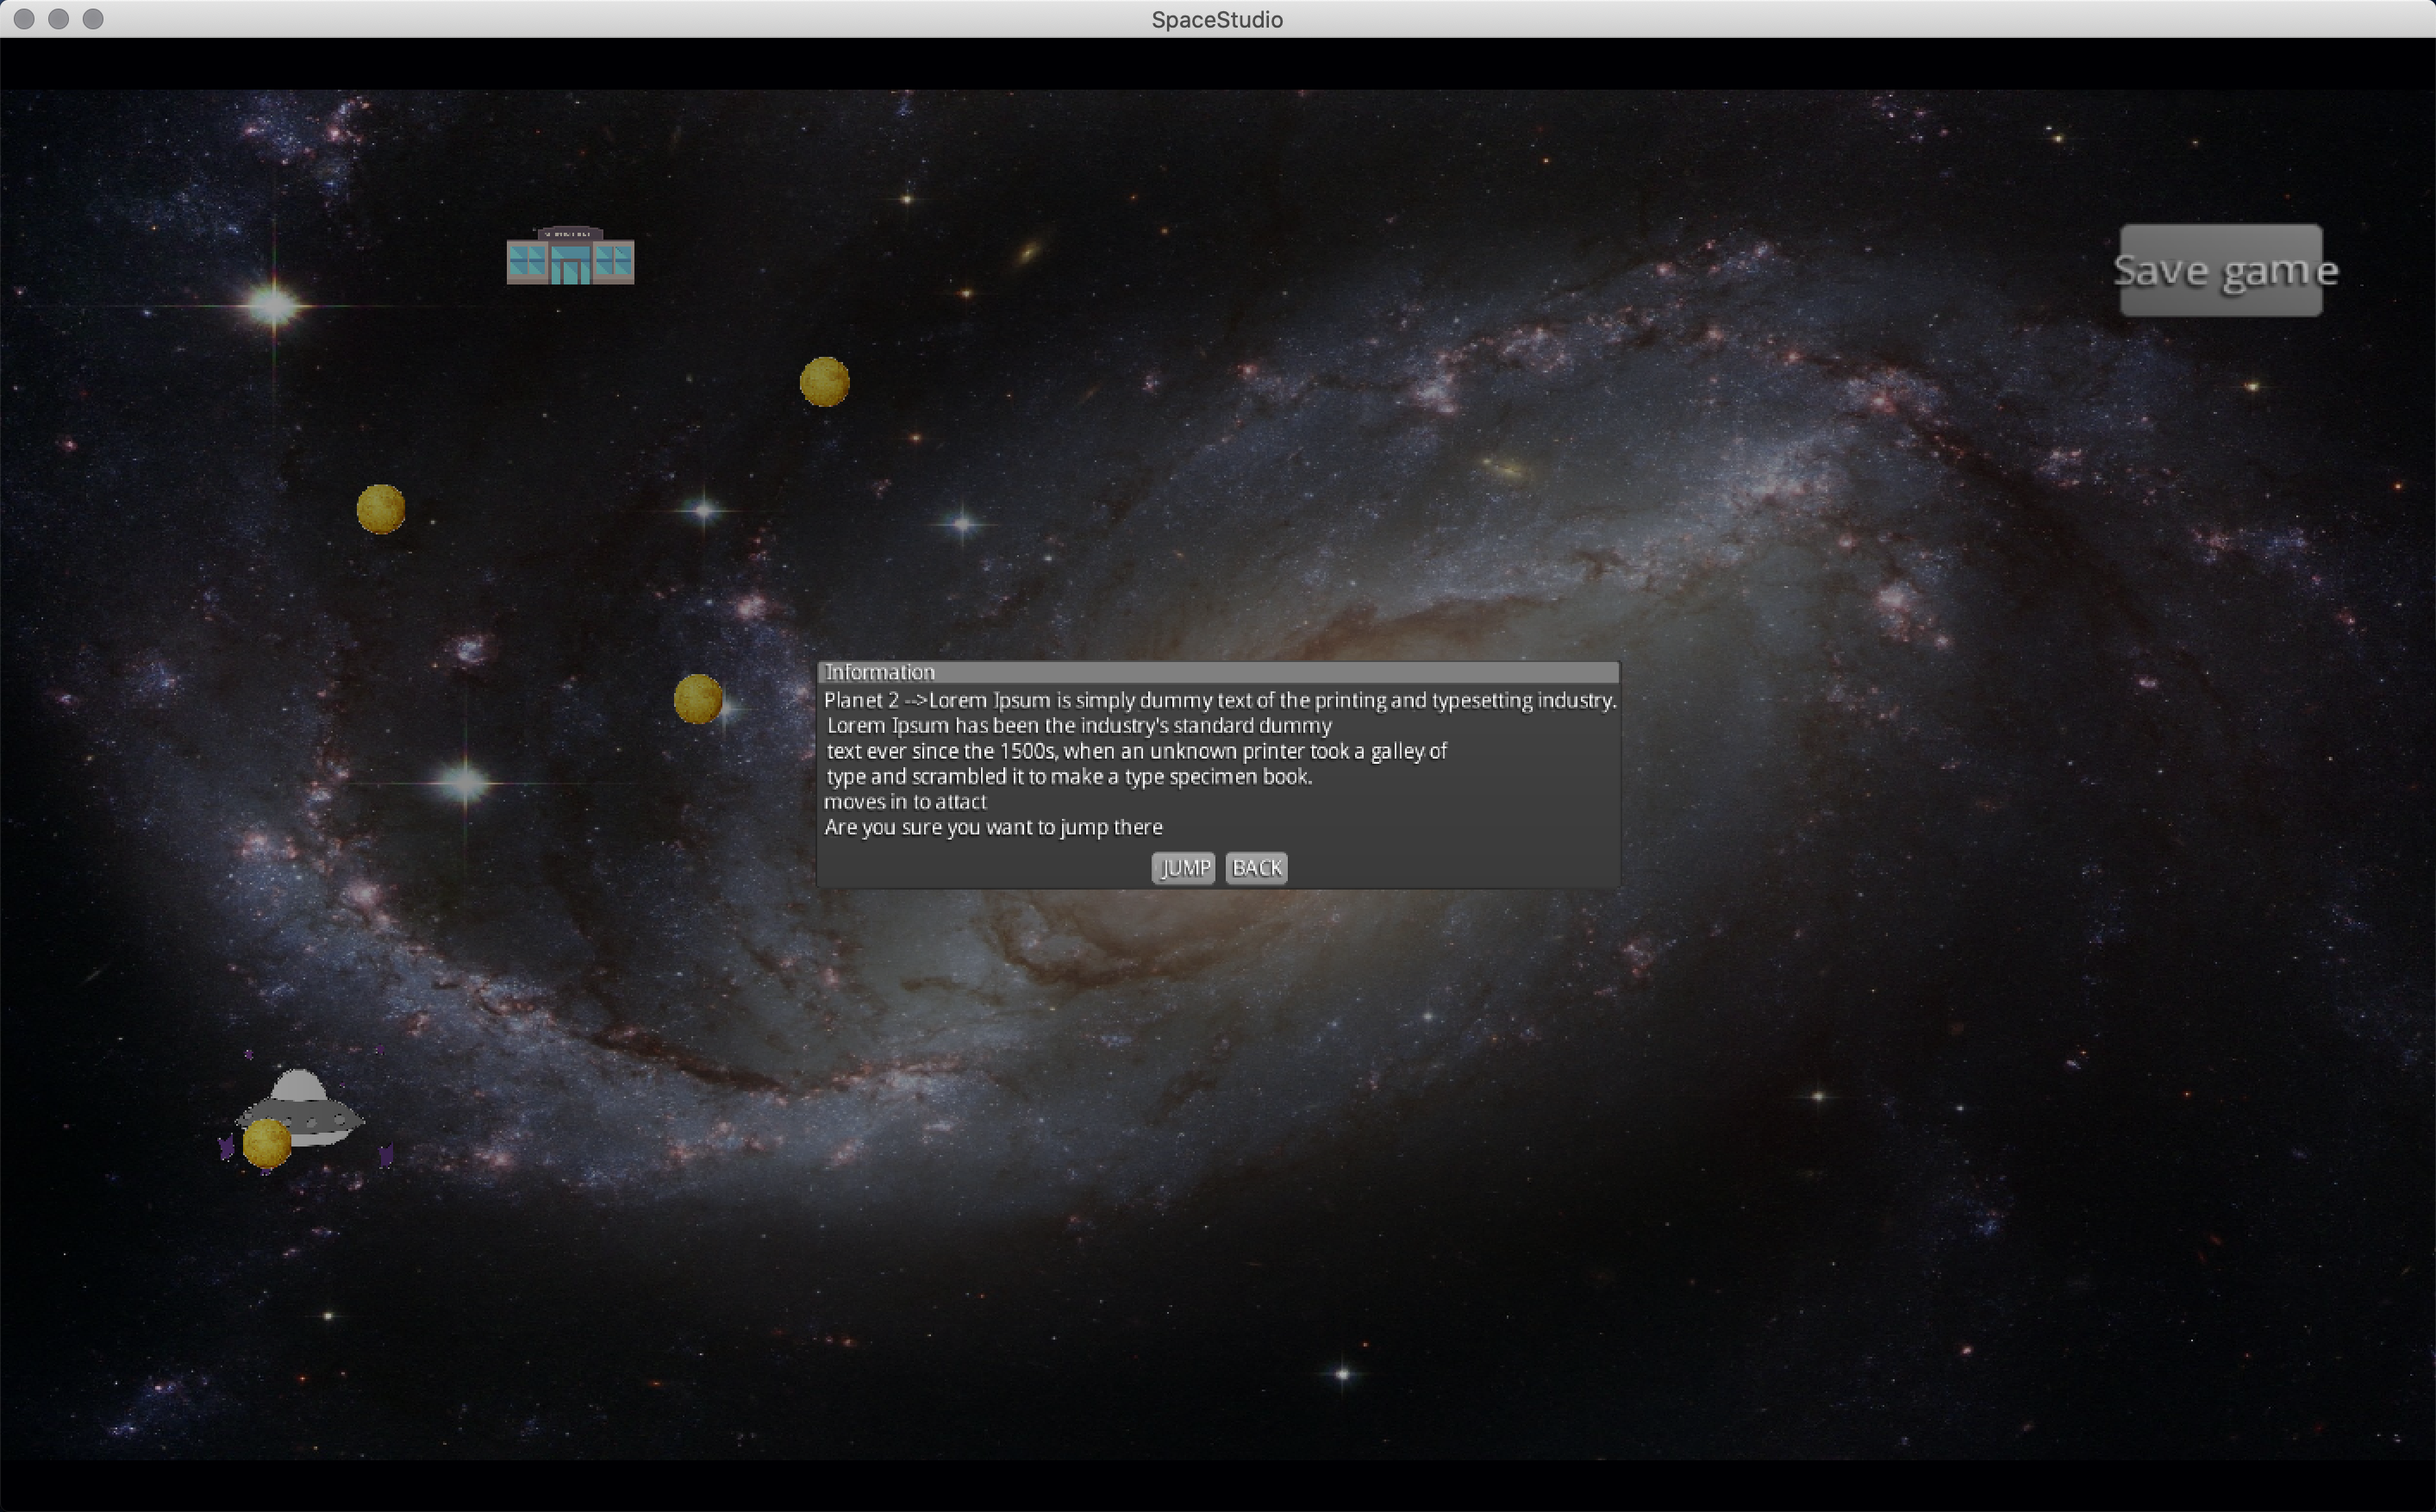
\includegraphics[scale=0.3]{TestProtocolBilder/jump.png}
\caption{Jump Buton}
\end{figure}
\newpage
Nach Auswahl der Sprungfunktion sieht der Benutzer auf dem Bildschirm eine Fahrzeit von 4 Sekunden.
\begin{figure}[htp]
\centering
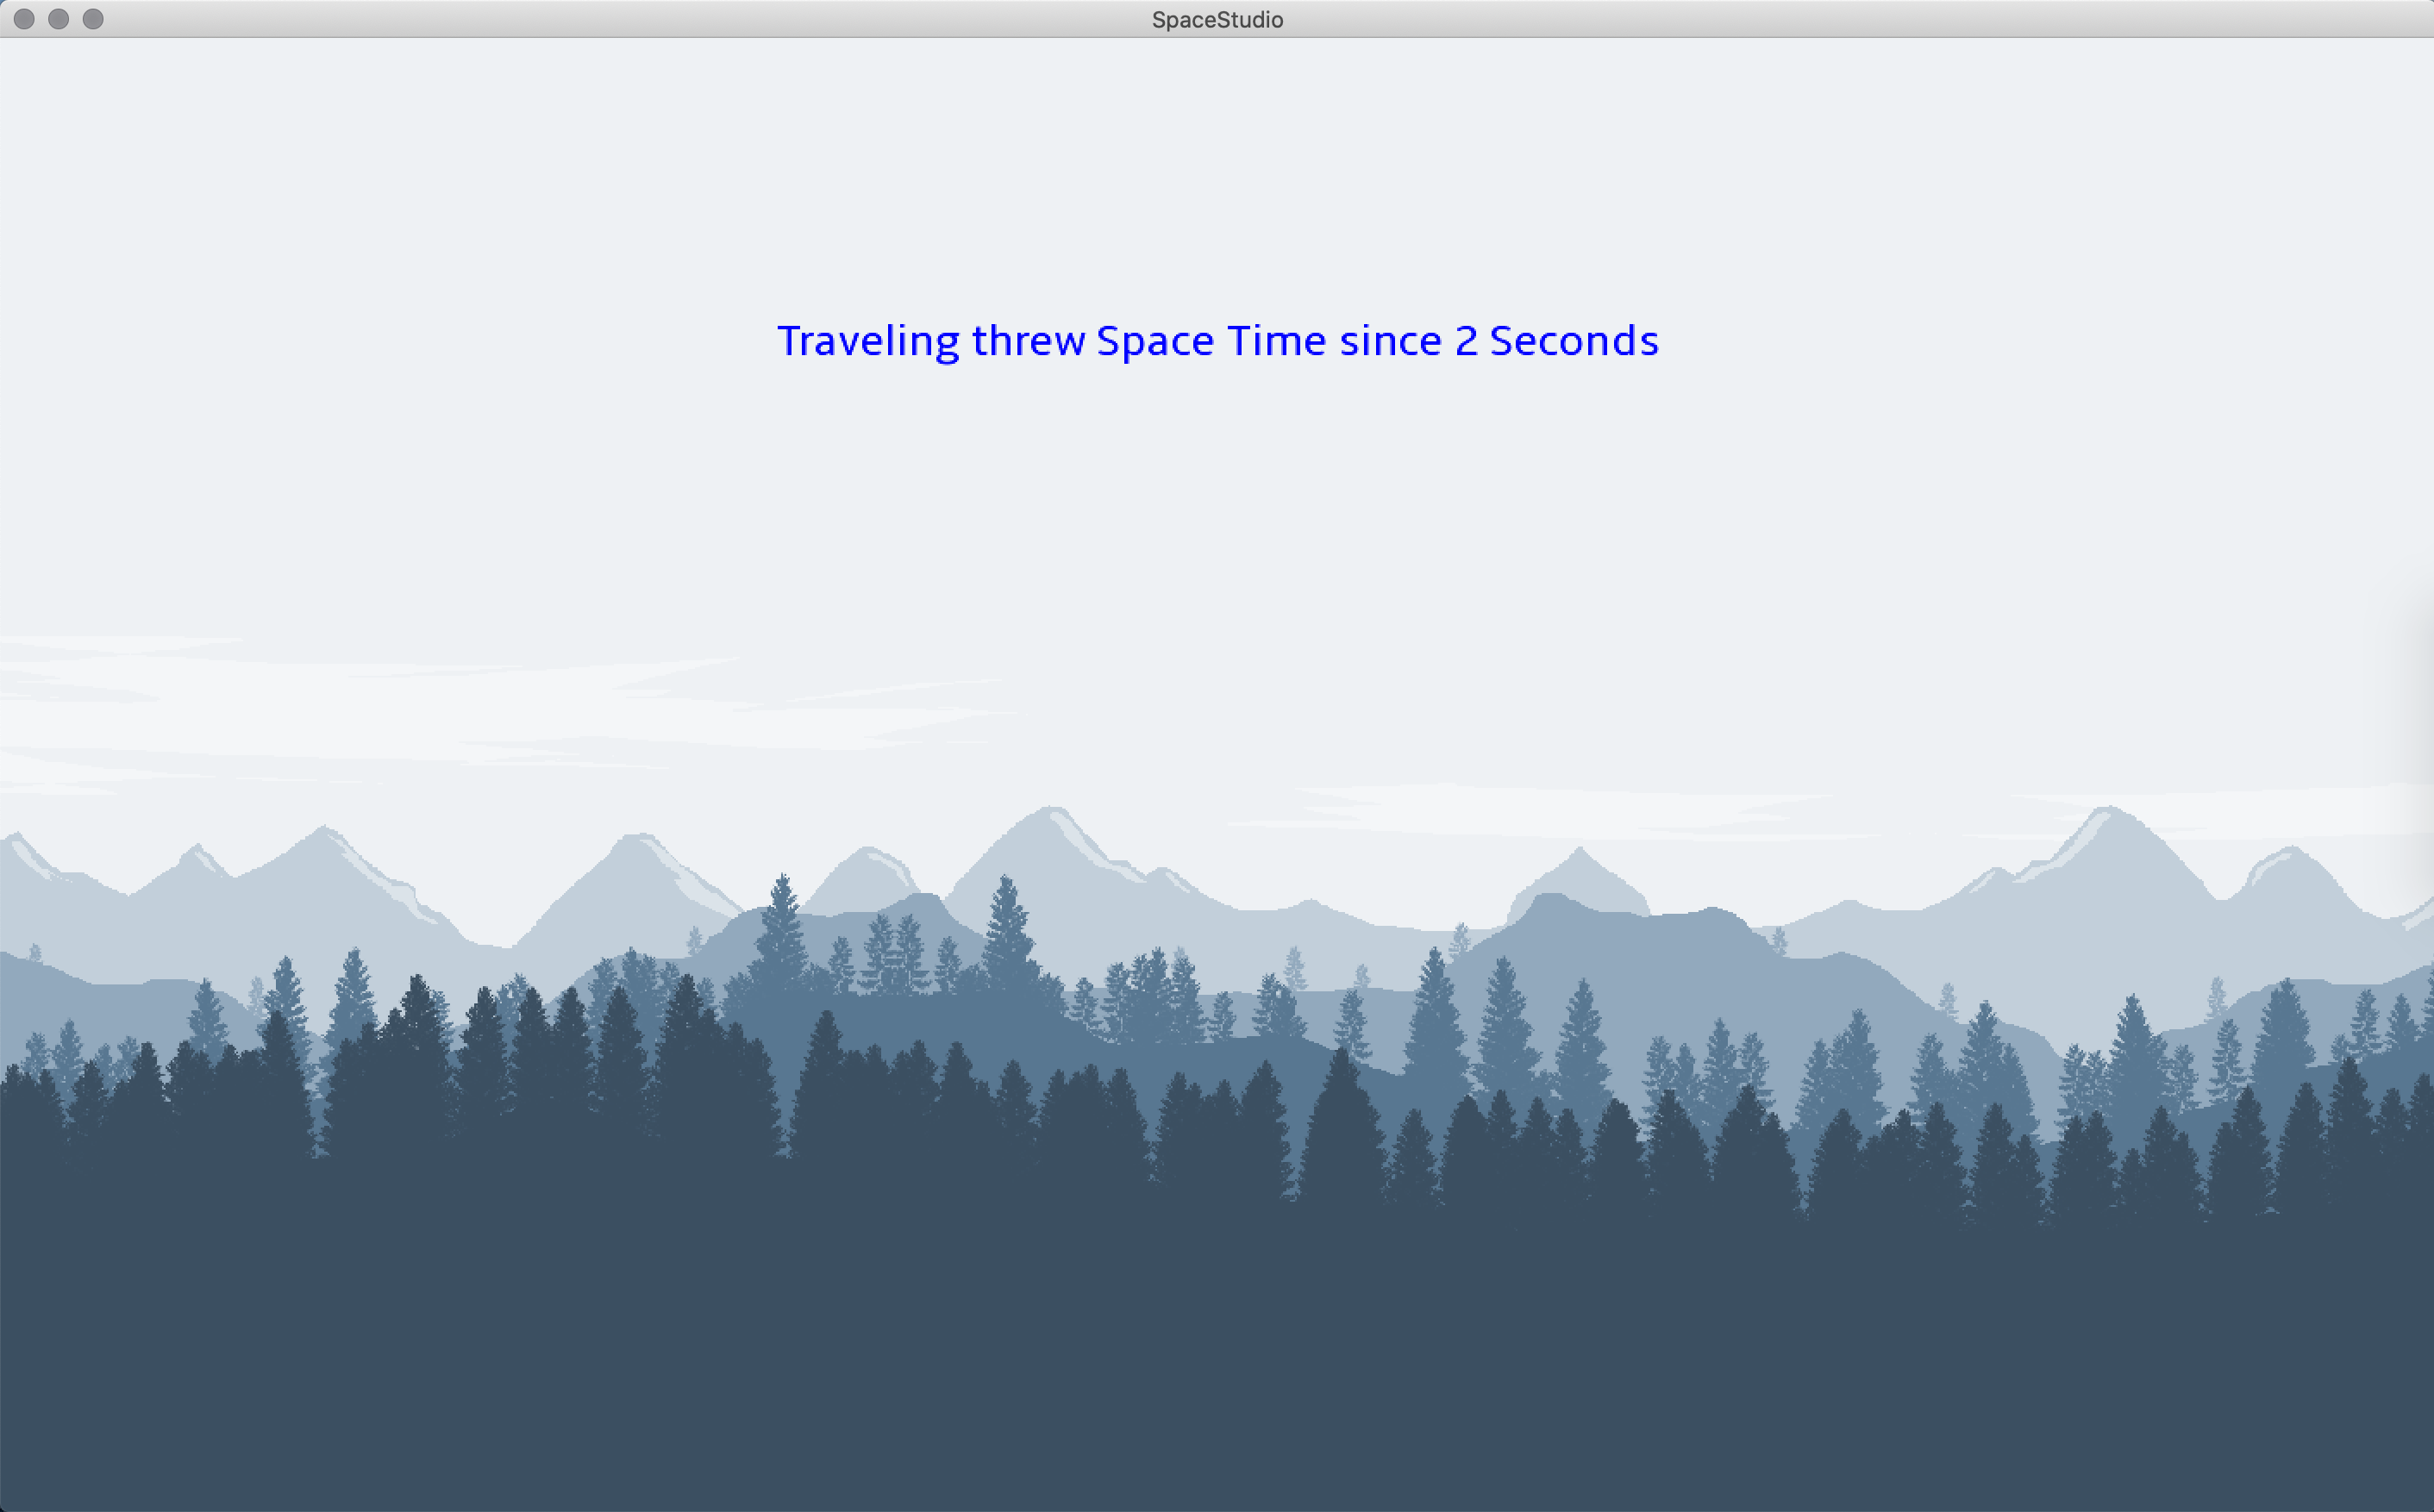
\includegraphics[scale=0.3]{TestProtocolBilder/traveling.png}
\caption{Traveling Screen}
\end{figure}
button flee test, dann man kann wieder an der Map Jump Springen.
\begin{figure}[htp]
\centering
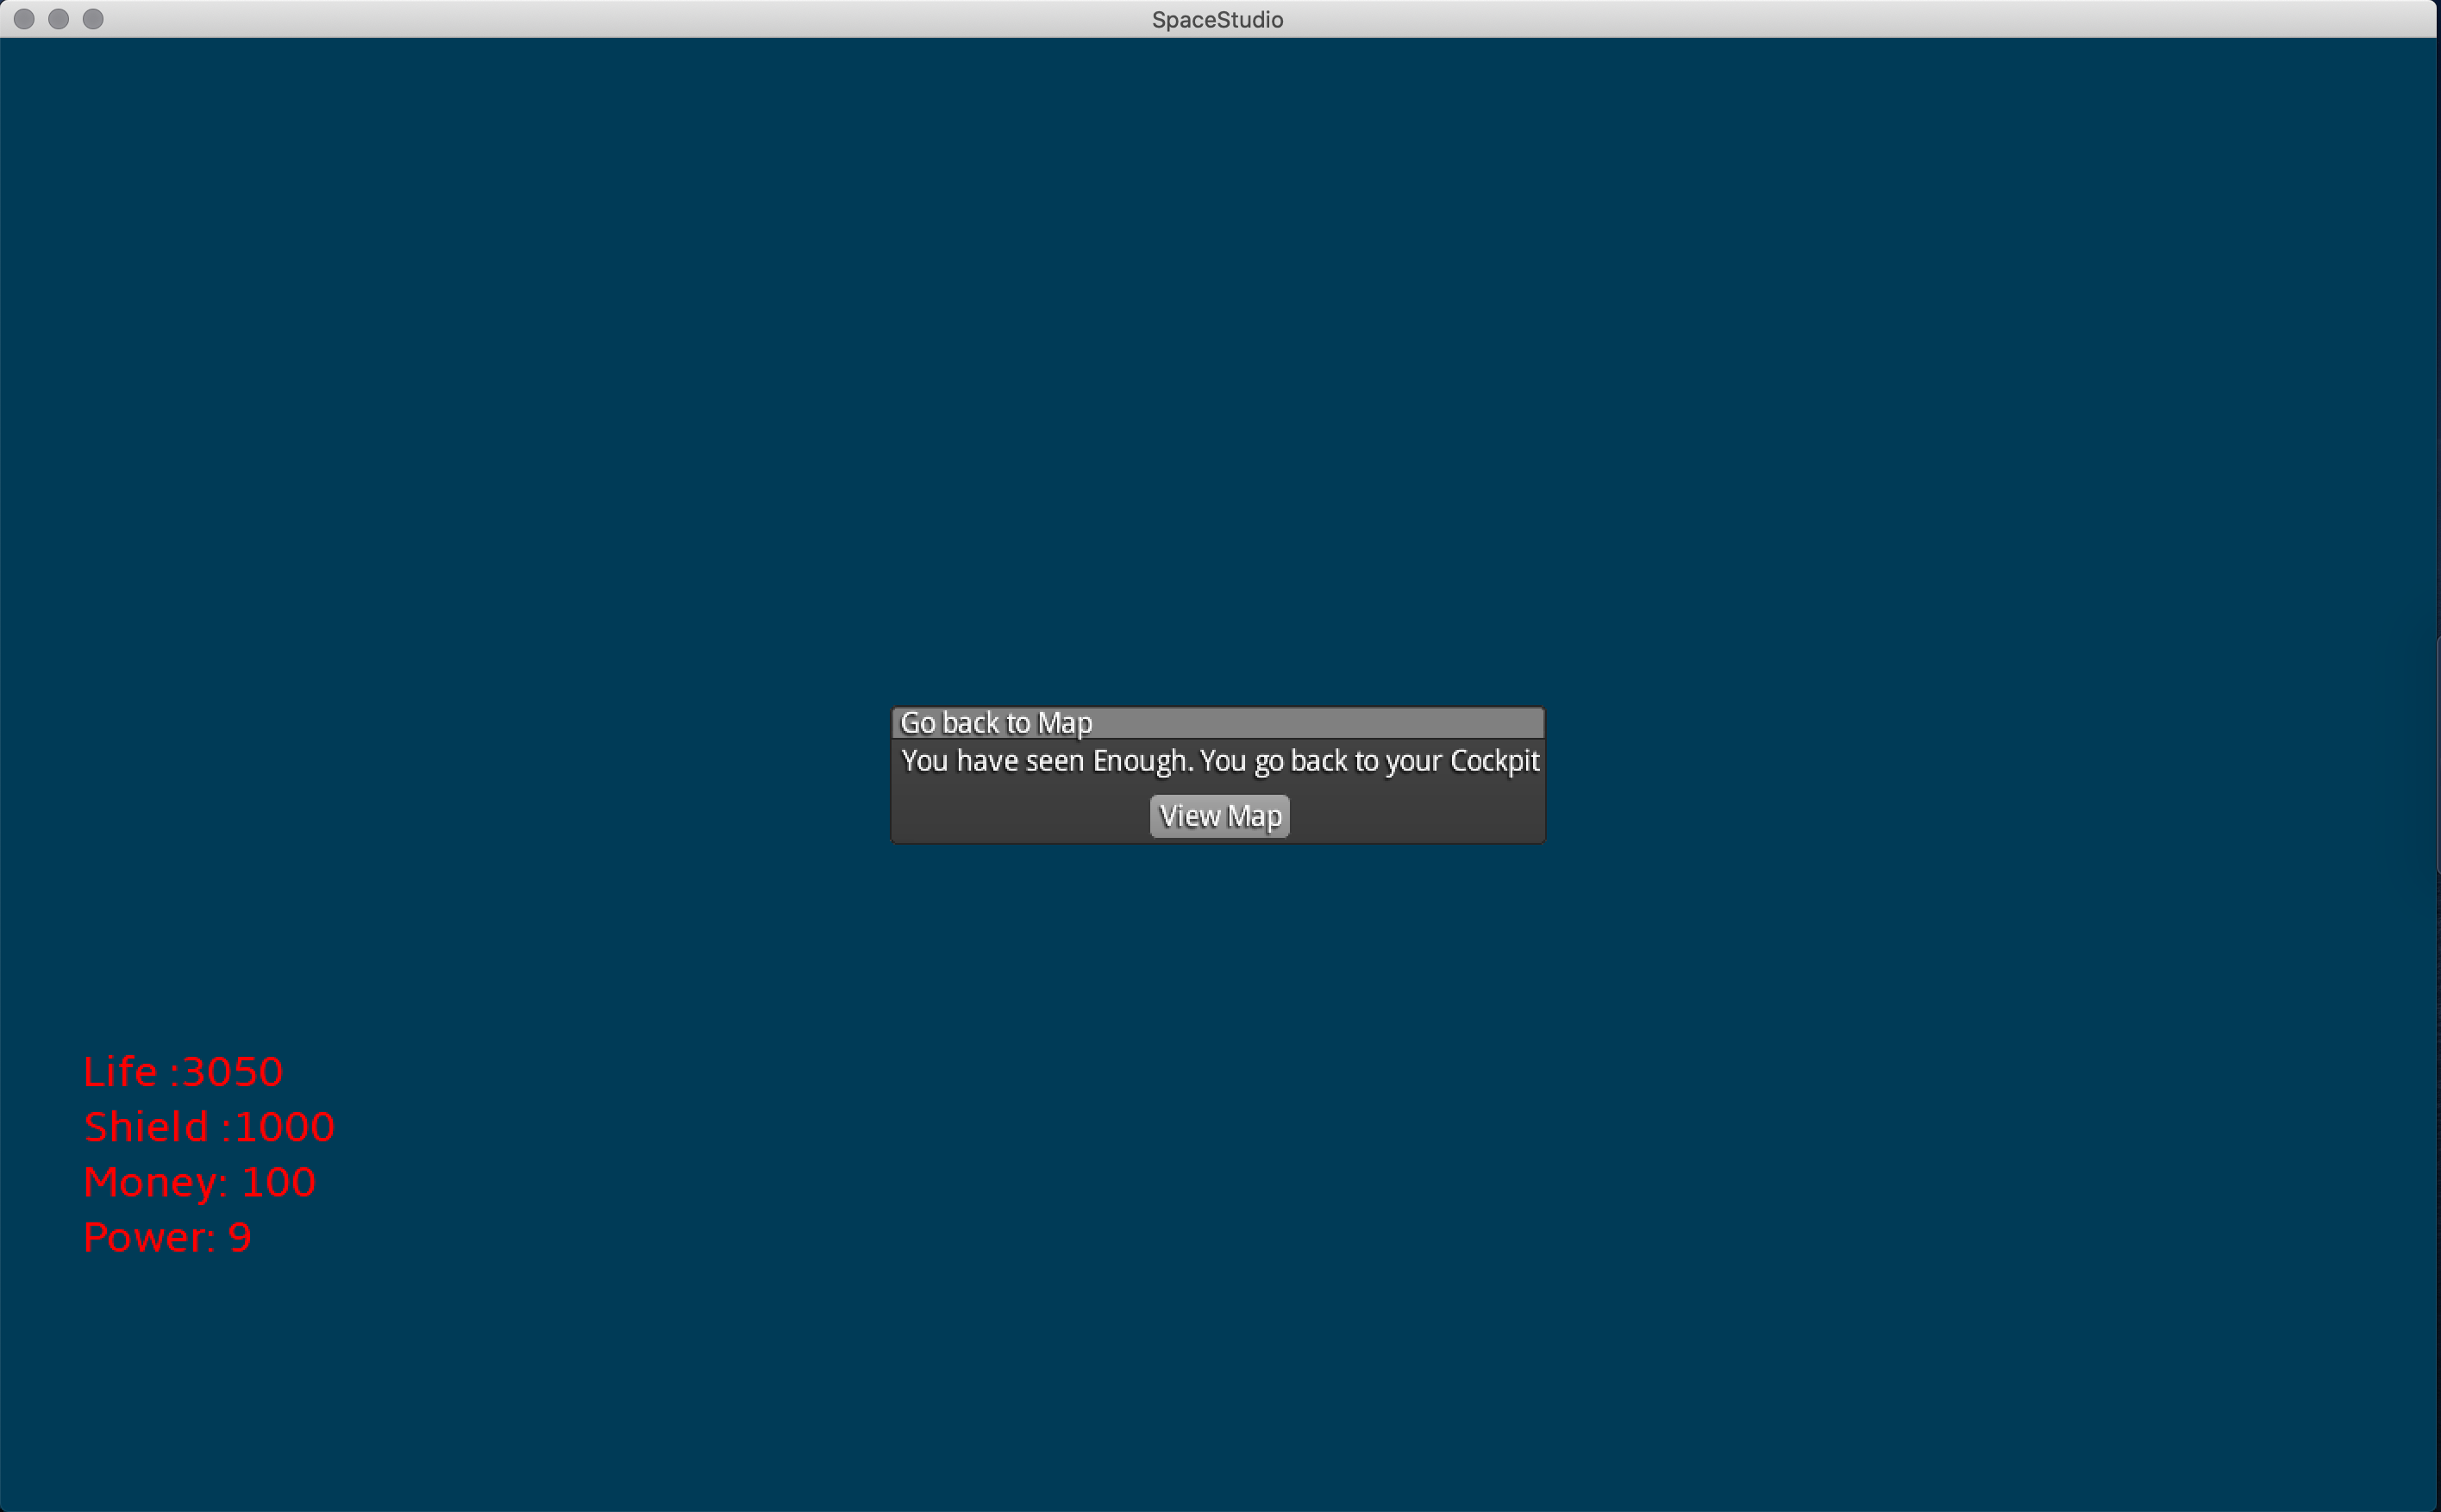
\includegraphics[scale=0.3]{TestProtocolBilder/flee.png}
\caption{Traveling Screen}
\end{figure}
\newpage
Es wurde getestet, dass nach dem Reisebildschirm der erste Teil der Ereignisse angezeigt wird.\\
\begin{figure}[htp]
\centering
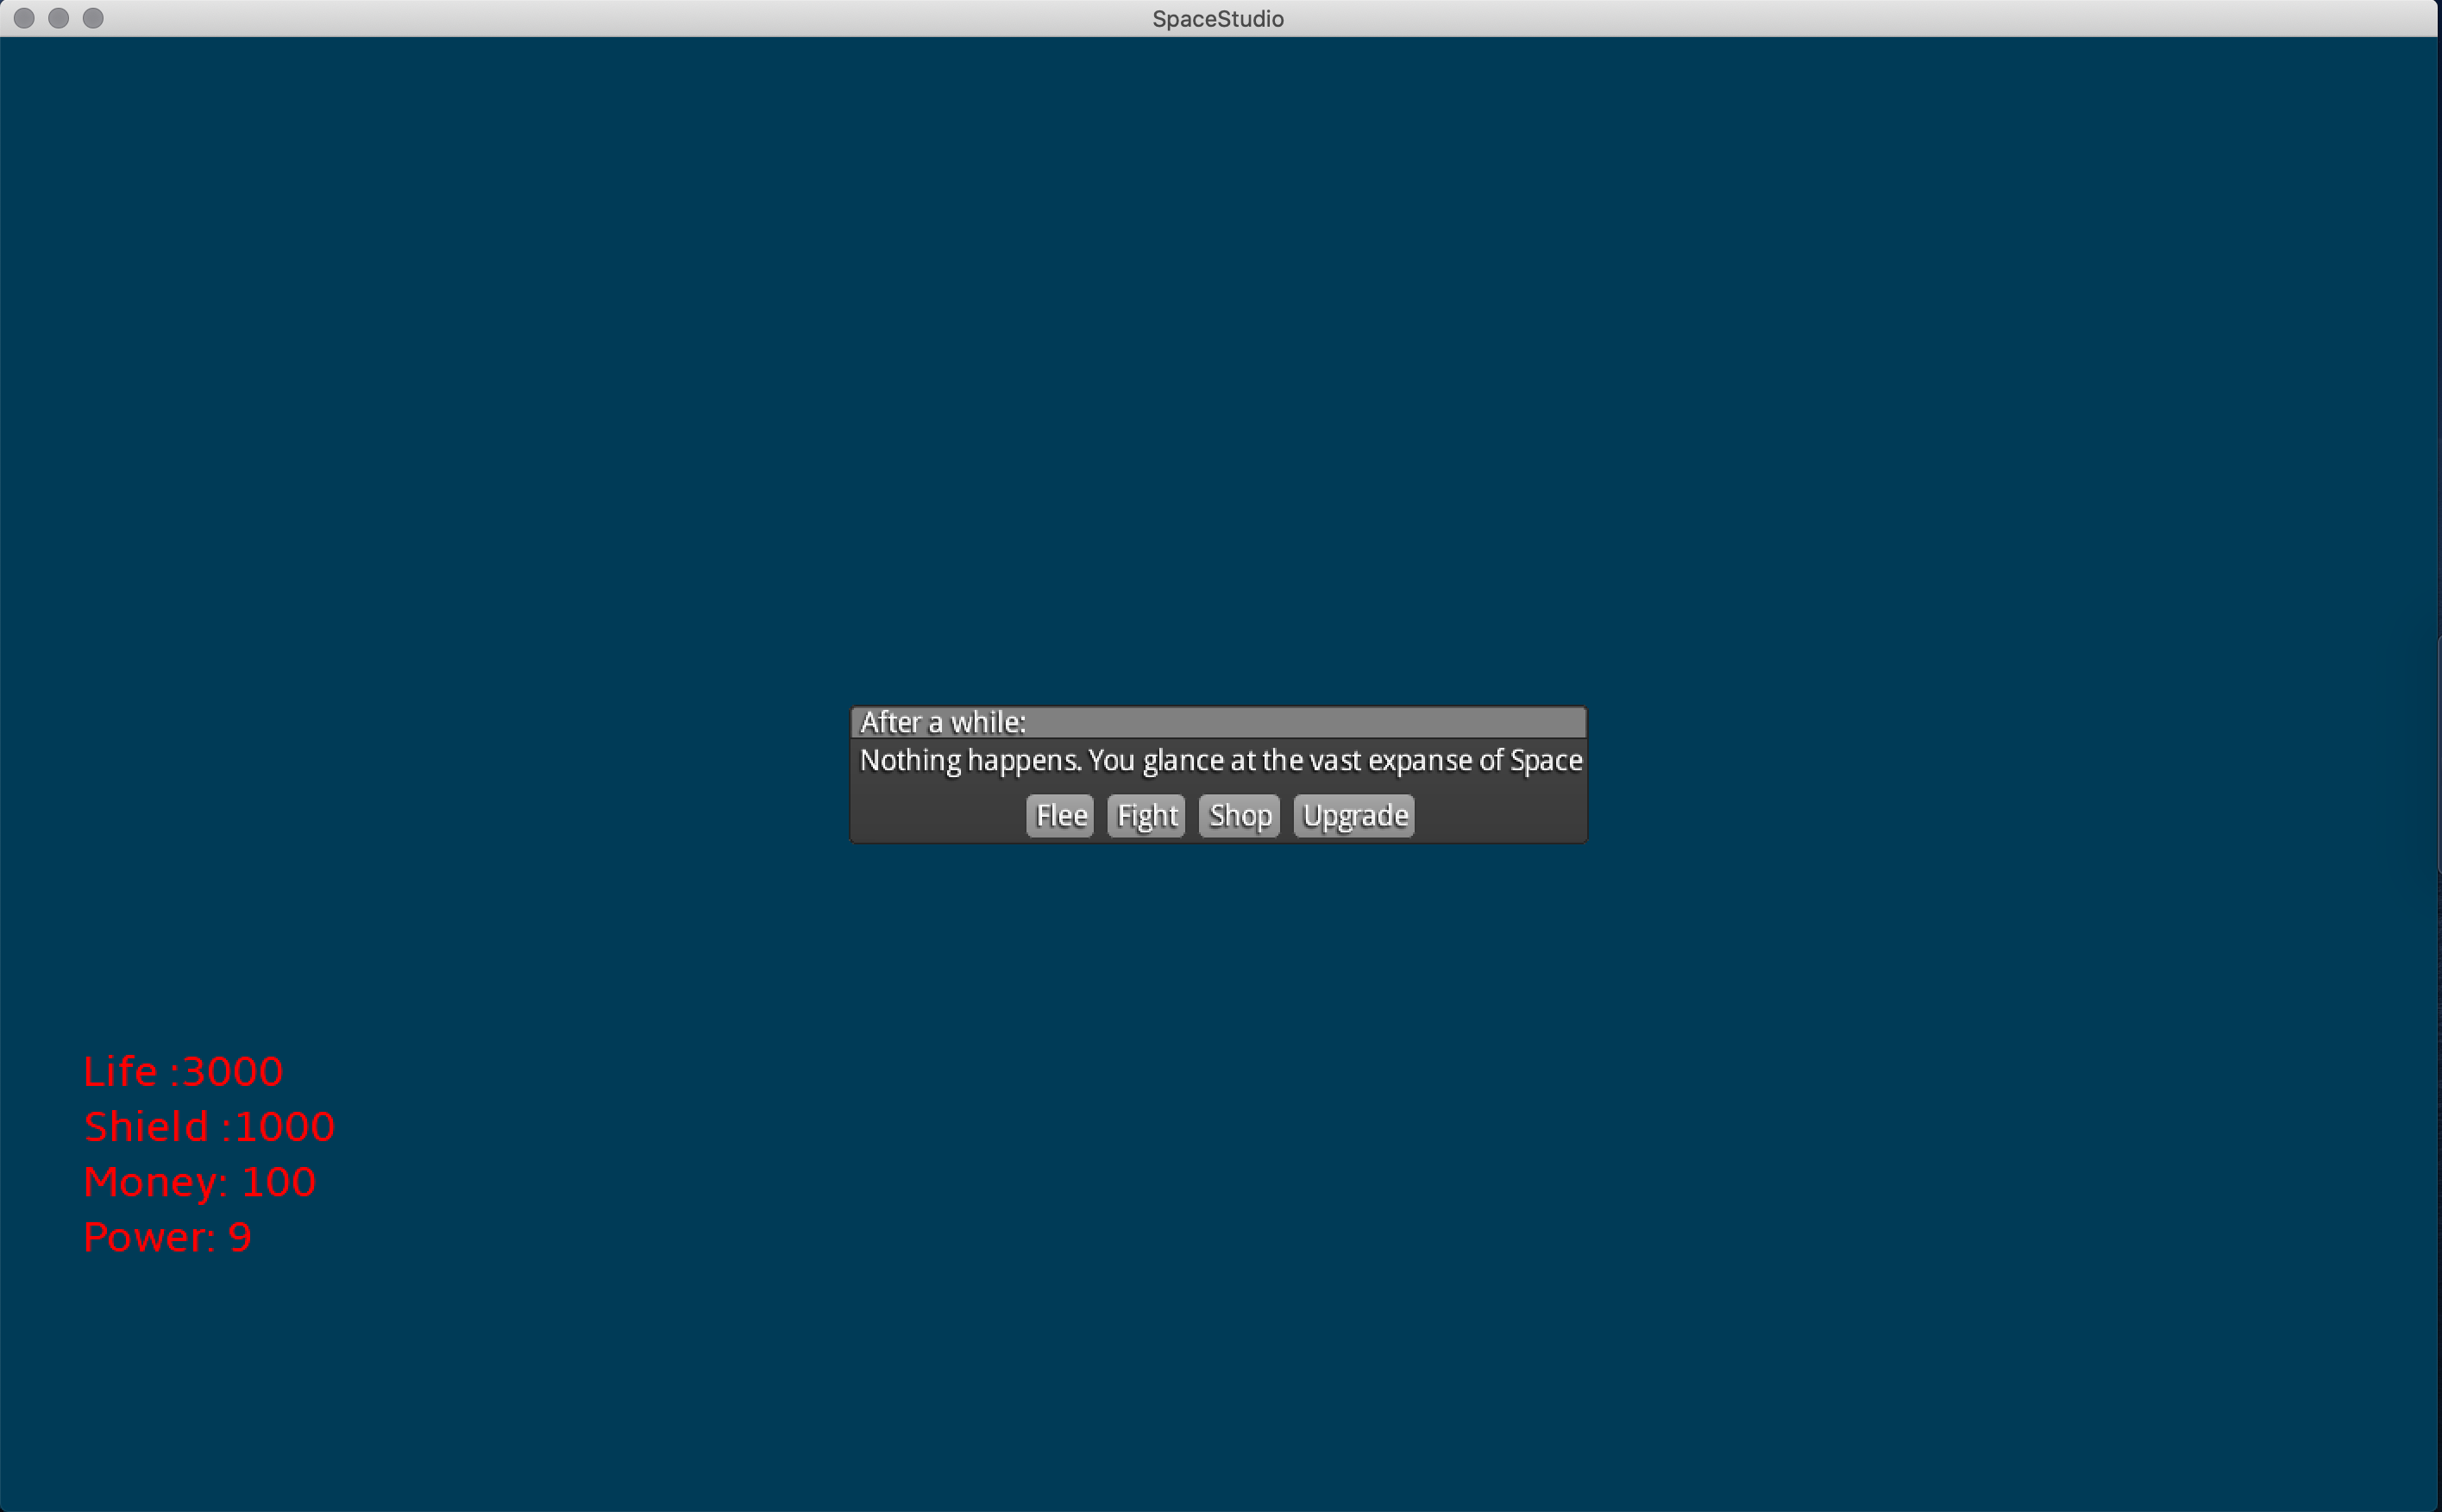
\includegraphics[scale=0.3]{TestProtocolBilder/InitialGeeinisse.png}
\caption{First Ereignisse}
\end{figure}
Dieser Bildschirm war für die Einführung des Benutzers in die Ereignisse gedacht.
\newpage


\begin{figure}[htp]
\centering
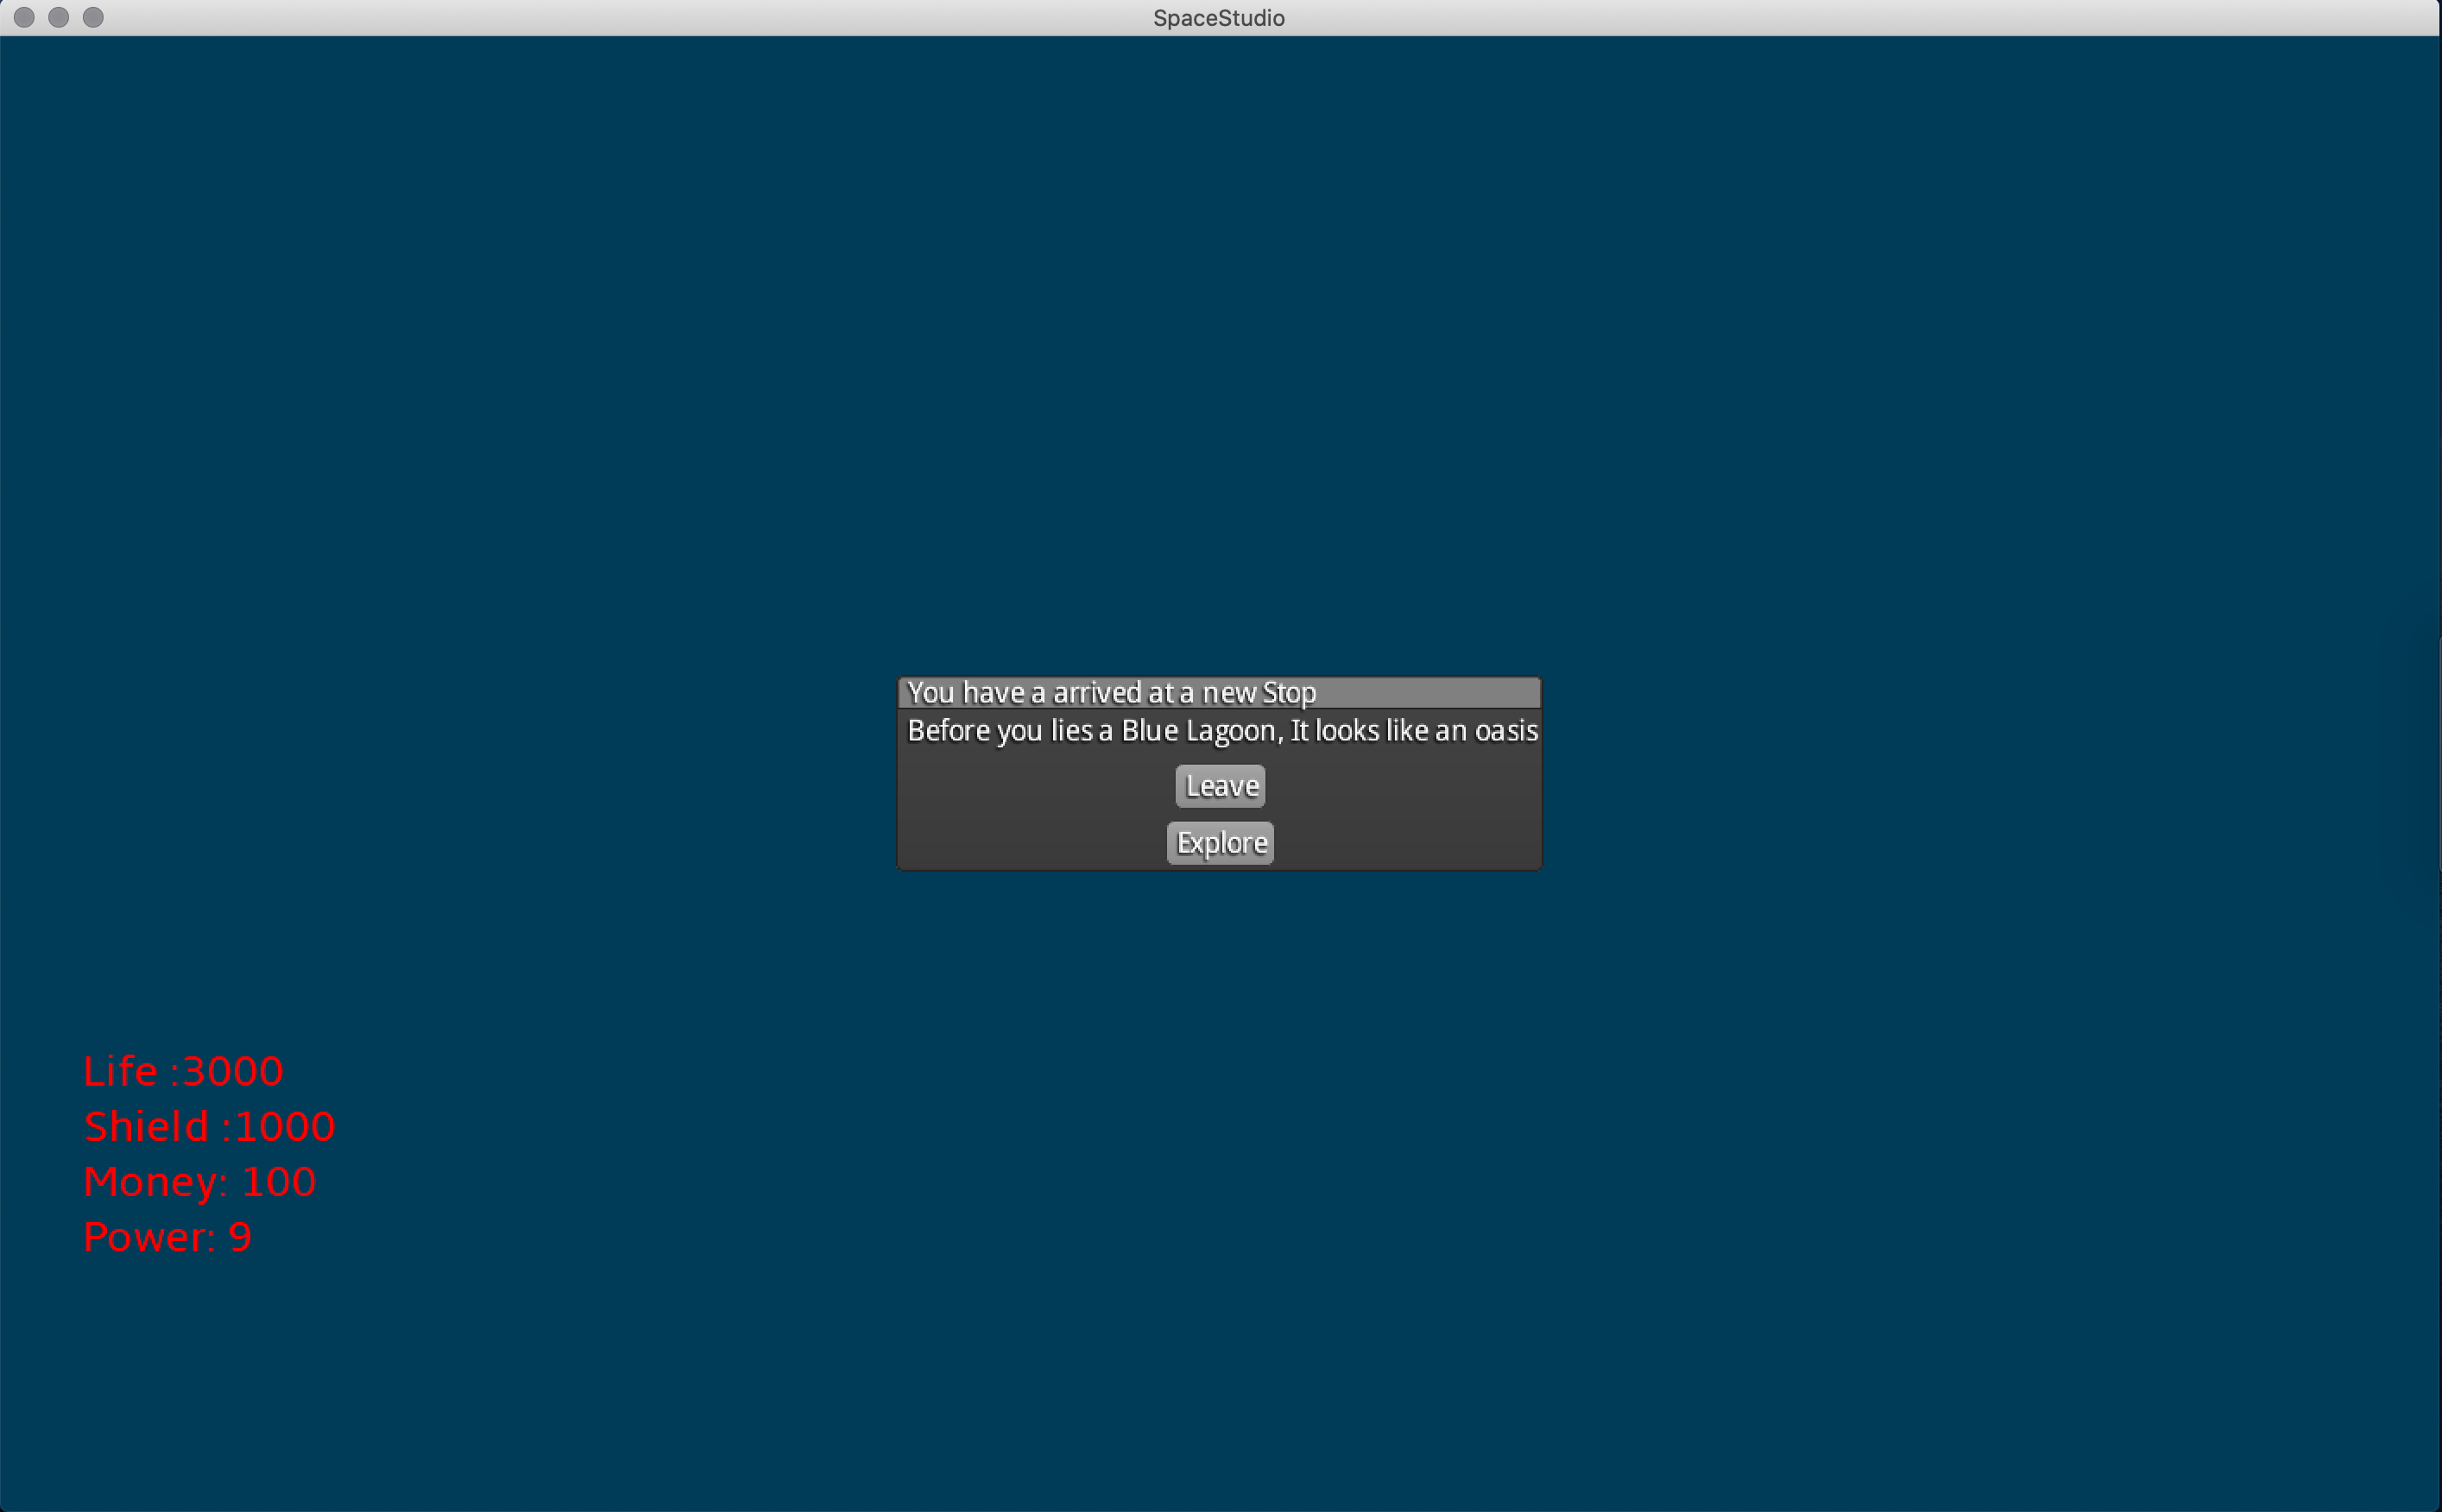
\includegraphics[scale=0.3]{TestProtocolBilder/otherEreignisse.png}
\caption{andere Typ von Ereignisse}
\end{figure}
\subsubsection{Goes back to Station Map}
\subsubsection{Goes back to Shop}


\subsubsection{Single Player (Ship Select Screen)}

\subsubsection{Are the Stats Updated for the Ship?}
\subsubsection{Can I spawn into the Map?}
\subsubsection{Are there Any Exceptions?}



\section{Station Screen}
\label{sec:orga891bce}

\subsection{StationMap}

\subsubsection{Select Planet}

\subsubsection{Can I select every Planet?}
\subsubsection{Does the Dialog Appear?}
\subsubsection{ Jump}
\subsubsection{Jump can I jump to every Planet?}
\subsubsection{Do I see if I have visited the Planet?}
\subsubsection{ Does the Back Button work?}


\section{Stop Abstract}
\label{sec:org3bde3ec}

\subsection{StopScreen}

\subsubsection{Leave}

\subsubsection{Leave}
\subsubsection{View Map -> Station Map}

\subsection{Explore}
\subsubsection{Flee -> Station Screen}
\subsubsection{Fight -> CombatScreen}
\subsubsection{Shop -> Station Mao}
\subsubsection{Back to Map -> Station Map}


\section{Combat Screen}
\label{sec:org9c941a6}
\subsection{Options}



\section{Strangenes}
\label{sec:org4b85c14}
\subsection{Rainbow Line}
\subsection{Pruebe Kopf in ShipSelectScreen}
\subsection{Bug Ship is not add at Stop}
\subsection{Jump to same Planet}

\end{document}